\documentclass[12pt,a4paper]{book}
\usepackage[T1]{fontenc}
\usepackage{textcomp}		% Companion symbols (useful to have)
\usepackage[utf8]{inputenc}
\usepackage[english]{babel}
\usepackage{lmodern}		% Uses the superior font

\usepackage{pdfx}			% Let's PDF/A it from the start
\usepackage{graphicx}		% For (you guessed it) including graphics

%% Cover-page-related
\usepackage[vcentering,dvips,left=4.0cm,right=3.0cm,top=3.5cm,bottom=3.0cm,includeheadfoot]{geometry}
%\geometry{textwidth=390pt}

%% Bibliography-related
\bibliographystyle{unsrt}
\usepackage{tocbibind}		% Adds bibliography (as well as figure and table lists)
							% to table of contents.

%% For better captions
\usepackage[font=small,labelfont=bf]{caption}
\usepackage{subcaption}

%% For SI units
\usepackage{siunitx}

%% Math related
\usepackage{amsmath}	% Matrix environments
\usepackage{amssymb} % \lesssim
\usepackage{mathtools} % Coloneqq, xrightarrow
\usepackage{braket} % Take a guess
\usepackage{dsfont} % For identity operator
\usepackage{bm}		% For bold math

%% For better tables (see https://people.inf.ethz.ch/markusp/teaching/guides/guide-tables.pdf)
\usepackage{booktabs}
\renewcommand{\arraystretch}{1.2}

%% This avoids page breaks in footnotes
\interfootnotelinepenalty=10000

%% To change the header
\usepackage{fancyhdr}
\pagestyle{fancy}

%% These change the display of \leftmark and \rightmark, for some reason
%% No, I have no idea what they do atm. Truly shameful
\renewcommand{\chaptermark}[1]{\markboth{#1}{}}
\renewcommand{\sectionmark}[1]{\markright{\thesection~~#1}}

\fancyhf{}

\setlength{\headheight}{15pt} %% Changes header height to accomodate text

%% E/O = even/odd pages
%% L/C/R = left/center/right alignment
%% H/F = header/footer
%% \thepage is page number
%% \leftmark is the chapter title
%% \rightmark is the section number and title
%% \nouppercase because otherwise bibliography comes up as BIBLIOGRAPHY in the header
\fancyhead[ELH]{\thepage}
\fancyhead[ORH]{\thepage}
%\fancyhead[ERH]{\leftmark}
\fancyhead[ERH]{\nouppercase{\leftmark}}
%\fancyhead[OLH]{\rightmark}
\fancyhead[OLH]{\nouppercase{\rightmark}}

%% This automatically makes math mode bold in chapter titles, I believe
\makeatletter
\g@addto@macro\bfseries{\boldmath}
\makeatother

%% Barn has been deprecated :( Fuck you Fermi
\DeclareSIUnit\barn{b}
\DeclareSIUnit\mev{\mega\electronvolt}
\DeclareSIUnit\gev{\giga\electronvolt}
\DeclareSIUnit\tev{\tera\electronvolt}
\DeclareSIUnit\rad{rad}
\DeclareSIUnit\mrad{\milli\rad}

%% For trailing space after shortcuts (otherwise it sticks to the next word)
\usepackage{xspace}
%% More shortcuts
\newcommand{\demonstratorfull}{$\Lambda_b^0 \rightarrow J/\psi~(\rightarrow \mu^+ \mu^-)~\Lambda^0~(\rightarrow p\pi^-)$\xspace}
\newcommand{\demonstratorshort}{$\Lambda_b^0 \rightarrow J/\psi~\Lambda^0$\xspace}
\newcommand{\physbkgfull}{$B^0 \rightarrow J/\psi~(\rightarrow \mu^+ \mu^-)~K^0_S~(\rightarrow \pi^+\pi^-)$\xspace}
\newcommand{\physbkgshort}{$B^0 \rightarrow J/\psi~K^0_S$\xspace}
\newcommand{\lz}{$\Lambda^0$\xspace}
\newcommand{\lbz}{$\Lambda_b^0$\xspace}
\newcommand{\jpsi}{$J/\psi$\xspace}
\newcommand{\pim}{$\pi^-$\xspace}
\newcommand{\slab}{$\text{S}_\text{L}$\xspace}
\newcommand{\shad}{$\text{S}_H$\xspace}
\newcommand{\slambda}{$\text{S}_\Lambda$\xspace}
\newcommand{\slambdal}{$\text{S}_{\Lambda\text{L}}$\xspace}
\newcommand{\lambdadecay}{$\Lambda^0 \rightarrow p\pi^-$\xspace}

%%%%%%%%%%%%%%%%%%%%%%%%%%%%%%%%%%%%%%%%%%%%%%%%%%%%%%%%%%%%%%%%

\begin{document}

%%%%%%%%%%%%%%%%%%%%%%%%%%%%%%%%

\frontmatter

%% Cover page
\newgeometry{centering}	% Make the page centered on paper
%\title{\textsc{Verso la misura del flusso di neutrini da CNO: Analisi radiale del fondo $^{210}$Bi-$^{210}$Po nel rivelatore Borexino}}
%\author{Alessandro De Gennaro}
%\date{2018}


\begin{titlepage}
	\begin{figure}[t]
		\centering
		
\includegraphics[width=390pt]{graphics/cover-page/logo.jpg}
		\centering
	%	\vspace{0.1 cm}
	\end{figure}	
\begin{center}
{\large Corso di Laurea Magistrale in Fisica}
\end{center}

\begin{center}
\vspace{2 cm}
{\Large \textsc{A study for the measurement of the $\Lambda$ baryon electromagnetic
dipole moments in LHC}b\par}
\end{center}
%\par
  \vspace{2 cm}
  
  \begin{flushleft}
  		 Relatore: \hskip 0.62 cm Prof. Nicola NERI\\
		 
  		 \noindent Correlatore: \hskip 0.1 cm Dott.ssa\ Elisabetta SPADARO NORELLA
  \end{flushleft}
  \vspace{1 cm}
  \begin{flushright}
  	Tesi di Laurea di:\\ Alessandro DE GENNARO\\ Matricola \hskip 0.1 cm 933289\\ Codice P.A.C.S.: \hskip 0.1 cm 14.20.-c
  \end{flushright}
    	  
%\vfill
\begin{center}
\vspace{2 cm}
{\large Anno Accademico 2020--2021}
\end{center}
\end{titlepage}
\restoregeometry		% Restore the page layout as earlier

\chapter*{Introduction}
\addcontentsline{toc}{chapter}{Introduction}
\markboth{Introduction}{}

%Cose da dire:
%
%* SM ha buchi
%* EMDM sondano quei buchi
%* Come vogliamo misurare EMDM noi
%* Come è ripartita la tesi

From the discovery of dark matter in spiral galaxies to the confirmation of neutrino oscillation as solution to the solar neutrino problem, evidence has piled up in favour of the incompleteness of the Standard Model of Particle Physics, currently the best description of particles at the subatomic level.
The subject of the violation of C and P discrete symmetries has gained traction in recent years to the ${10}^{-10}$ disparity between the known Standard Model sources of violation and the extent required to explain the present matter-antimatter asymmetry in the Universe. 

One promising pathway to new physics is the study of electromagnetic dipole moments of elementary and composite particles.
Permanent electric dipole moments (EDMs) introduce a CP-violating term in the system's Hamiltonian;
given that expected Standard Model contributions are orders of magnitude smaller than current experiment sensitivities, EDM upper limits place strict constraints on the existence of new physics.
Magnetic dipole moments (MDMs) can further be used to probe violation of the CPT theorem, which predicts MDMs to be the same for particles and matching antiparticles.

Electromagnetic dipole moments of long-lived particles can be measured from the precession of their spin-polarization vector in a strong magnetic field, which depends on the particle's gyroelectric and gyromagnetic factors.
In this thesis, I present my work in preparation of a measurement of the electromagnetic dipole moments of the \lz baryon with the LHCb experiment.
Long-lived \lz baryons from the exclusive \demonstratorfull decay are selected with the requirement that the \lz decay after the LHCb dipole magnet, allowing for the comparison of initial and final polarization states.
Theoretical background for the EDM/MDM measurement approach and specifics on the LHCb detecting apparatus are reported in Chapters \ref{cap:flavour_physics} and \ref{cap:LHCb} respectively.

%Electric and magnetic dipole moments of particles are sensitive to physics within and beyond the Standard Model. In this thesis, sensitivity studies for the measurement of the Lambda baryon electromagnetic dipole moments based on pseudo experiments will be performed. In addition, the possibility of a first measurement using data collected with the LHCb detector will be explored. 

For the first part of my thesis, detailed in Chapter \ref{cap:vertex_reconstruction}, I report on my work in understanding and improving the vertex reconstruction process in LHCb, with the main goal to mitigate the low efficiency of \lambdadecay reconstruction in \demonstratorshort events.
I also analyze the $z$ resolution of the reconstructed \lz vertex to gauge possible sources of bias.

In the second part of my thesis, I focus on the development and finalization of the three major steps in the signal selection process: preliminary filters, rejection of \physbkgshort physical background (including a newly-introduced \kshort veto based on the Armenteros-Podolanski technique), and discrimination of signal through the training and testing of a nonlinear multivariate classifier.
Results on this front are collected in Chapter \ref{cap:event_selection}.

Finally, in Chapter \ref{cap:angular_distribution} I capitalize on my earlier work to perform a first analysis of the angular distribution of \lambdadecay decay products, a key stepping stone in the prospective measurement of the \lz electromagnetic dipole moments.

%% Bring order to chaos. \chaptermark fixes uppercase letters in header
\tableofcontents
\chaptermark{Contents}
%\listoffigures
%\chaptermark{List of Figures}
%\listoftables 
%\chaptermark{List of Tables}

%%%%%%%%%%%%%%%%%%%%%%%%%%%%%%%%

\mainmatter
\chapter{Flavour physics and CP symmetry violation}
This chapter explores the theoretical framework for the rest of the thesis.
Section \ref{sec:sm} will provide a basic introduction to the Standard Model of Particle Physics and flavour physics in particular;
Section \ref{sec:discrete} will delve into the inner workings of discrete symmetries in quantum physics;
Section \ref{sec:edms} will discuss the relevance of electromagnetic dipole moments of elementary particles as a test for CP violation and CPT symmetry;
finally, Section \ref{sec:lambda} will introduce the main topic of the thesis, the study of dipole moments of the $\Lambda$ baryon.

\section{The Standard Model of Particle Physics}
\label{sec:sm}
Ever since Democritus' philosophy of atomism, one of the driving desires behind mankind's advancements in the fields of natural science has been to reduce reality to its basic components.
While one can convincingly argue that we may never fully understand what has come to be known as the quantum world, the Standard Model of Particle Physics (Standard Model, or SM, for short) is as close as physics has to offer to a comprehensive theory of the building blocks of matter and energy.

[... Qualcosa sulle previsioni sperimentali confermate.]

While the Standard Model is a self-consistent theory tested to a high degree of precision, it would be a serious mistake to call it \textit{complete}, even if only for the three fundamental forces it covers.
Many experimental evidences, some of which will be discussed in the following pages, have already opened cracks in the model, and many more are likely to emerge in the future;
one of the recurring topics of this chapter will thus be the need for physics Beyond the Standard Model (BSM).

\subsection{Elementary particles}
\begin{figure}[t!]
	\centering
	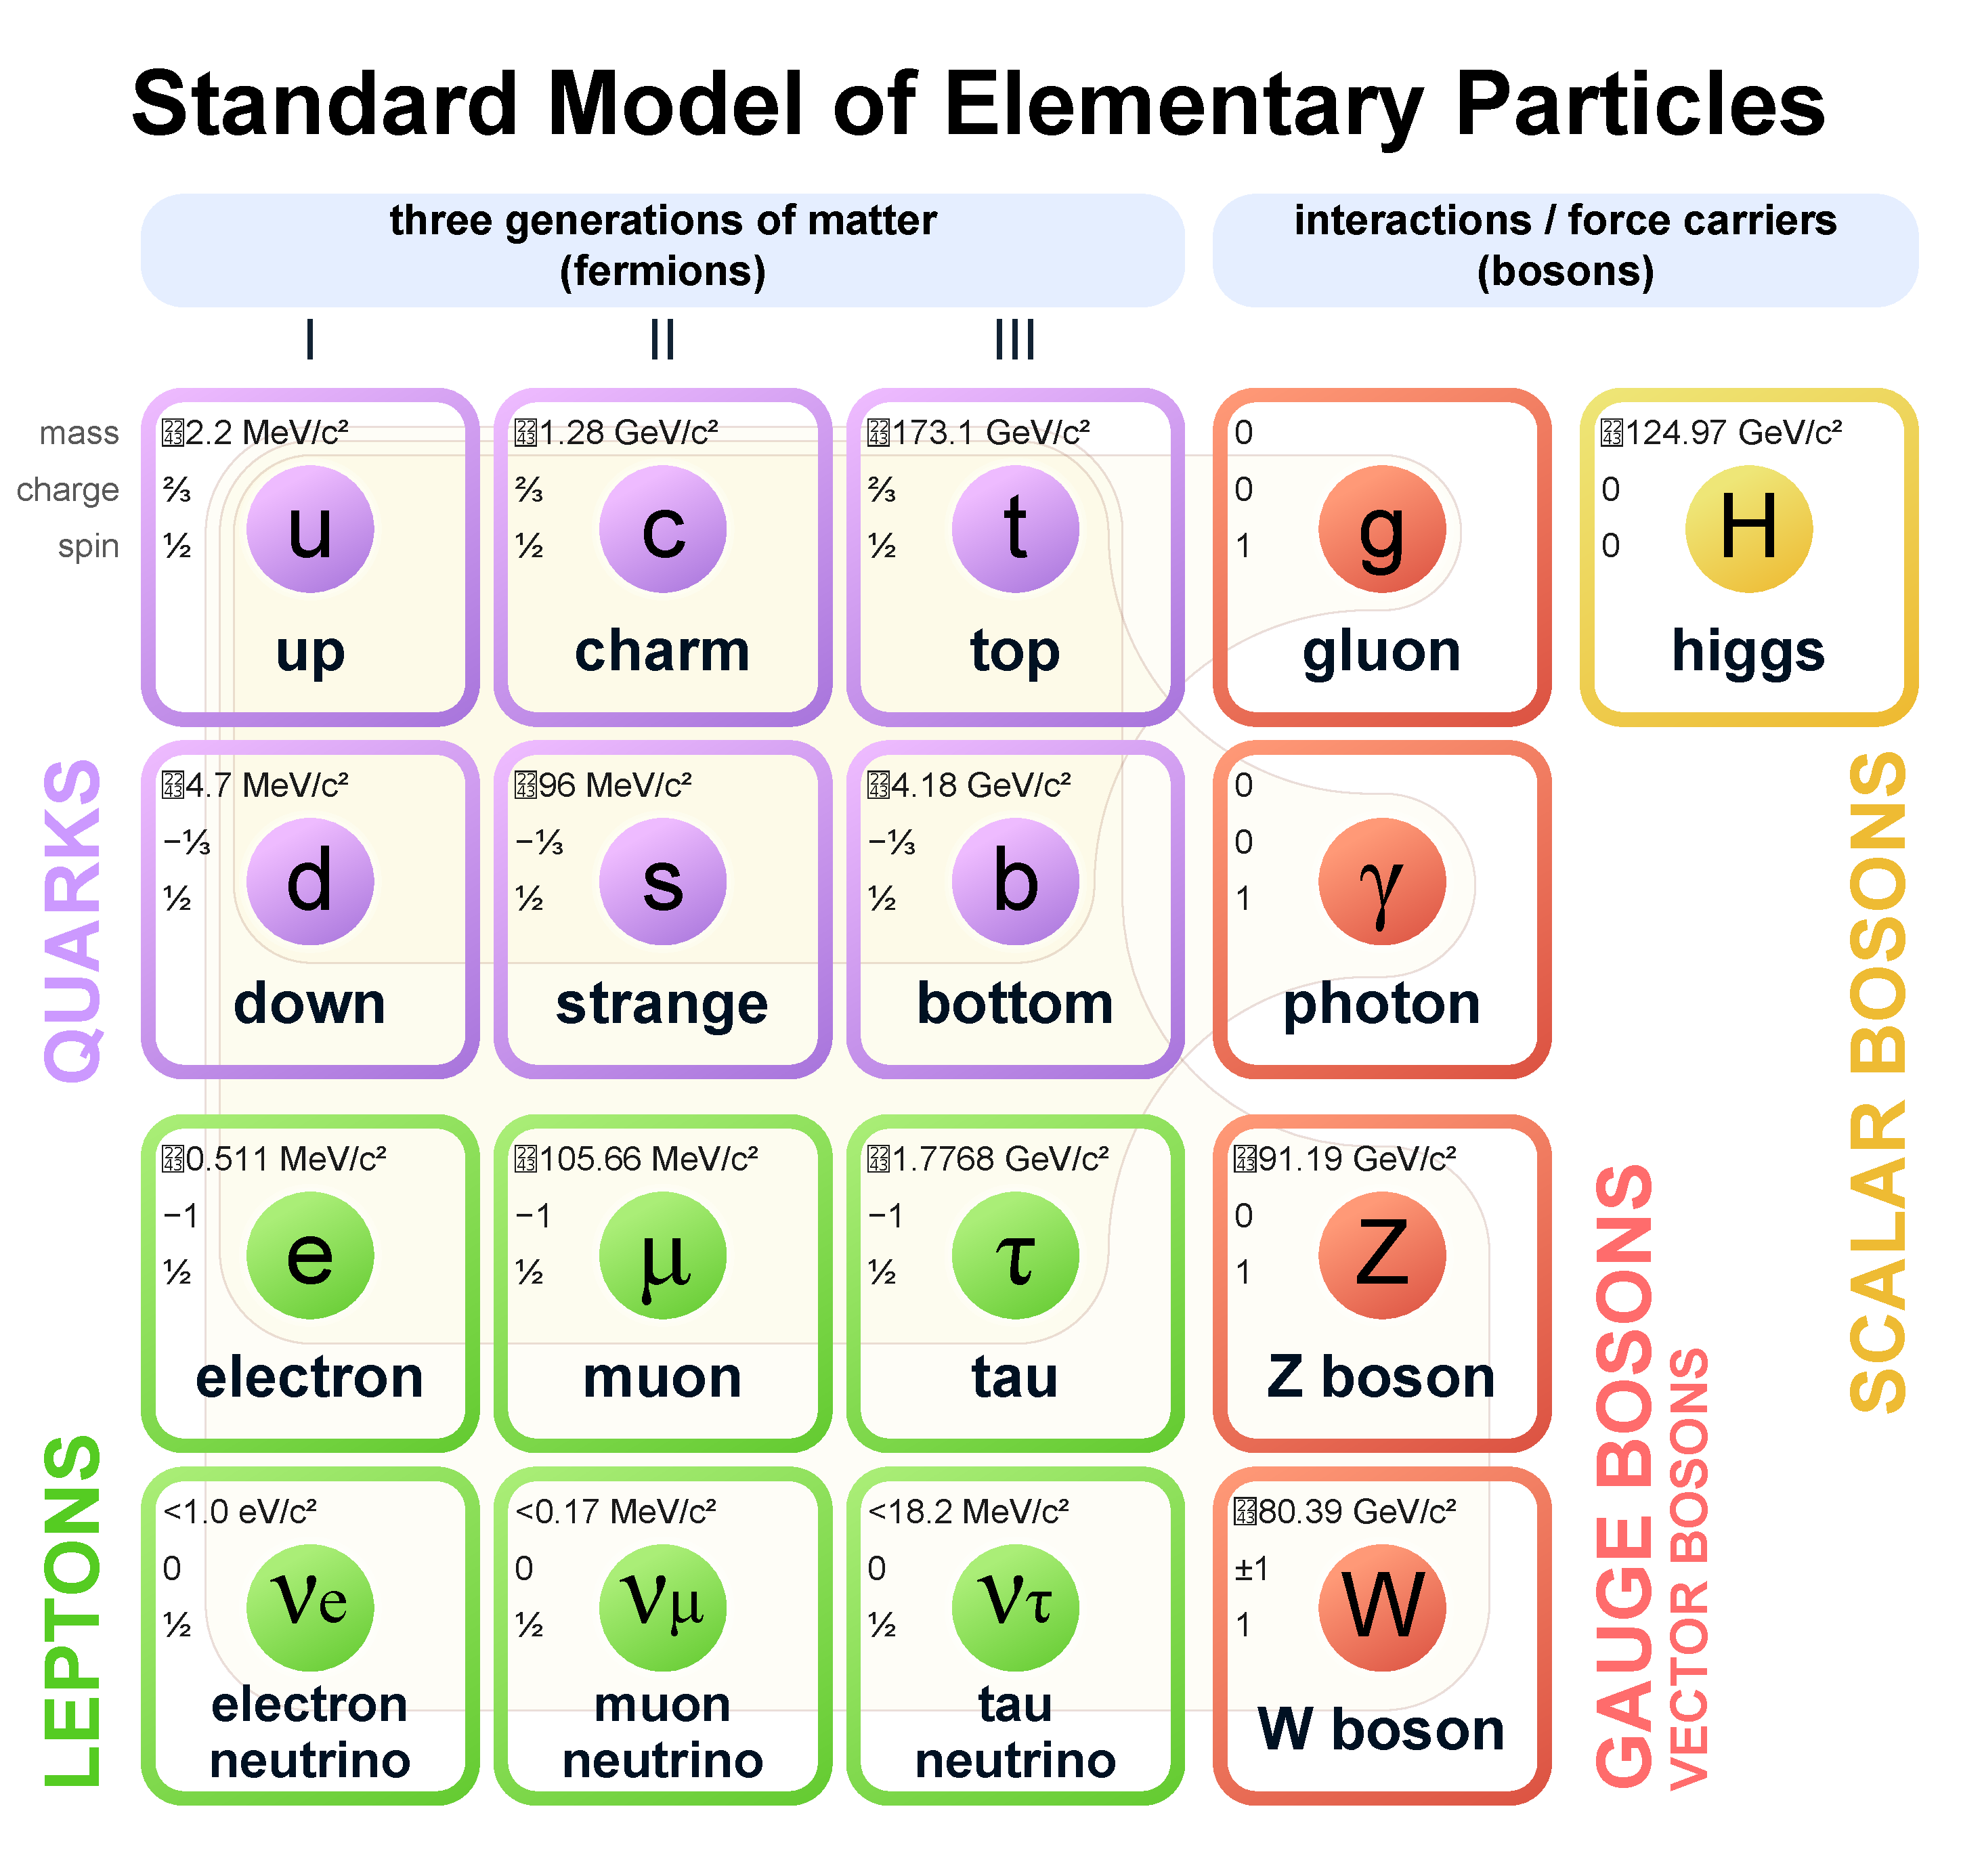
\includegraphics[scale=0.15]{graphics/01-standard_model/Standard_Model_of_Elementary_Particles.pdf}
	\caption[Currently known Standard Model elementary particles.]{The seventeen currently known elementary particles of the Standard Model. Antiparticles are not depicted.}
	\label{fig:particle_zoo}
\end{figure}

Intuitively, a particle is said to be \textit{elementary} when no substructure can be probed. 
A century of efforts in the fields of nuclear, quantum, and high energy physics has whittled down the spectrum of matter to just seventeen unique fundamental particles, colloquially known as the \textit{particle zoo} and depicted in Figure \ref{fig:particle_zoo}.

Each particle is joined by an \textit{antimatter particle} (\textit{antiparticle} for short), a companion of opposite charge identified by the prefix \textit{anti-}, e.g. antimuon for the muon; the only exception to this naming convention is the electron, whose antiparticle, for historical reasons, is known as positron.
While often omitted for the sake of brevity, antiparticles are elementary particles in every respect, distinct from their partners (bar the neutral gauge bosons, which are their own antiparticles) and related to them through the transformation of charge conjugation (see Section \ref{sec:C-symmetry}).

\subsubsection{Leptons}
Leptons are fermions (half-integer spin particles) not sensitive to the strong nuclear interaction.
There are currently six \textit{flavours} of leptons grouped in three generations: each generation comprises a \textit{charged} lepton (electron, muon, tauon) and a \textit{neutral} lepton (electron neutrino, muon neutrino, tauon neutrino).

All charged leptons have a charge of $-e$, where $e$ is defined as the \textit{elementary positive charge}, and their mass ranges from $\approx \SI{0.5}{MeV}$ for the electron to over $\SI{1.7}{GeV}$ for the tauon.
By contrast, as the names suggest, all neutrinos are electrically neutral and are assumed massless in the Standard Model\footnote{The observation of flavour oscillation in solar neutrinos shows that neutrinos do in fact have non-zero, albeit very small, mass.}; this implies that their only meaningful interactions happen through the weak nuclear force, which grants them their characteristic evasiveness to most particle detectors.


\subsubsection{Quarks}
Much like leptons, quarks are also fermions existing in three generations. The main difference from the former category is that quarks, besides interacting through weak and electromagnetic forces, are also susceptible to the strong nuclear forces; this allows them to bind together in composite states known as \textit{hadrons}, which are classified as \textit{baryons} (states of three quarks) and \textit{mesons} (states of one quark and one antiquark)\footnote{As recently as 2003, evidence has surfaced for the existence of exotic baryons composed of four (\textit{tetraquarks}) and five quarks (\textit{pentaquarks}).}.

Quarks can be classified as \textit{up-type} (up, charm and top quarks) and \textit{down-type} (down, strange and bottom quarks): up-type quarks have a fractionary charge of $+\frac{2}{3} e$, whereas down-type quarks have a charge of $-\frac{1}{3} e$. All quarks also have one of three \textit{color} charges (red, green or blue), while antiquarks similarly have one of three \textit{anti-color} charges (antired, antigreen or antiblue). A combination of all three colors/anti-colors or a combination of a color and its matching anticolor produces \textit{colorless} particles, a property of all observed quark composite states.

Unlike leptons, quarks are impossible to observe directly: according to the phenomenon of \textit{color confinement}, the energy of the interaction field between two color charges being pulled apart increases with their distance until it becomes high enough to create a quark-antiquark pair.
This process of \textit{fragmentation} develops many times over in such a way that the final observable state is entirely composed of colorless particles.
For this reason, high energy physics experiments such as LHCb do not detect free quarks, instead observing cone-shaped streams of hadrons known as \textit{hadronic jets}.

\subsubsection{Gauge bosons and fundamental interactions}
In quantum field theory, the interaction between two fields is implemented through the exchange of an intermediary particle known as \textit{force carrier}.
In the Standard Model all force carriers are vector (spin $1$) bosons known as \textit{gauge bosons}, the name being owed to the \textit{gauge principle} used to introduce them: the localization of a global continuous symmetry group provides the free fermion Lagrangians with interaction terms with the proviso that one or more bosonic fields are introduced.

%The fundamental forces driving the interactions between elementary particles are introduced in the Standard Model via the so-called \textit{gauge principle}, which adds an interaction term to the free Lagrangian as a result of the localization of a global continuous symmetry group; accordingly, the related force carriers are known as \textit{gauge bosons}.

The gauge principle accounts for the implementation of three fundamental interactions along with their gauge bosons: 
the \textit{strong nuclear force} with its massless gluon, responsible for the binding of both quarks inside baryons and nucleons inside atomic nuclei; the \textit{electromagnetic force} mediated by the massless photon, the importance of which should be known from everyday life; and the \textit{weak nuclear force} with two massive $W^\pm$ and $Z$ bosons, the source of many subnuclear processes such as $\beta$ radioactivity.

The latter two forces share a unified description in the Glashow-Weinberg-Salam theory as a single \textit{electroweak interaction} and are introduced via localization of a $\text{SU(2)}_L \otimes \text{U(1)}_Y$ symmetry group, the first related to the conservation of weak isospin in left-handed chirality states and the second to the conservation of hypercharge.
Quantum chromodynamics (QCD), the theory of the strong nuclear force, is based on a separate $\text{SU(3)}_C$ symmetry acting on the three-dimensional space of color charges.

There are no gauge bosons nor gauge theories associated to the fourth known fundamental force, gravity.
Since every attempt to reconcile the general theory of relativity with quantum mechanics has failed so far, gravity is presently excluded from the Standard Model;
this doesn't affect SM predictions at the subatomic level on account of the remarkably low intensity of said force, over 30 orders of magnitude lower than the weak interaction.

\subsubsection{The Higgs boson}
The Higgs boson is one of the latest additions to the Standard Model, being proposed in 1964 and observed by the ATLAS and CMS collaborations in 2012.
Its introduction solved perhaps the most insidious SM shortcoming at the time: gauge theories, which the model was built on, only worked under the assumption that all particles involved were massless, whereas the local invariance would fall apart (\textit{gauge breaking}) when adding a free mass term.

By contrast, the Higgs field accounts for mass generation of the weak bosons $W^\pm$ and $Z$ via the Brout-Englert-Higgs mechanism resulting from the spontaneous electroweak symmetry breaking;
elementary fermions also gain mass through a distinct, Yukawa-like interaction with the field.

\subsection{Flavour physics} \label{sec:flavour-physics}
A reader unfamiliar with SM terminology may find amusing the use of the word \textit{flavour} to refer to what have been so far presented as different kinds of particles altogether.
However quirky, the lexical choice highlights a defining feature: flavour, much like the degree of sweetness in a recipe, can change.

As often happens in particle physics, the rules are somewhat easier for leptons. For a given generation $\ell = (e,\mu,\tau)$, one can define a \textit{lepton family number} $L_\ell$ as the difference between the number of particles and antiparticles of said generation, charged leptons and neutrinos alike:
\begin{equation}
L_\ell
\coloneqq
n(\ell^-) - n(\ell^+)
+
n(\nu_\ell) - n(\bar{\nu}_\ell).
\end{equation}
For all three generations, $L_\ell$ is conserved in every interaction except neutrino oscillations.

Quarks are not as straightforward.
A similarly defined quark flavour number, such as the so-called \textit{topness} (or \textit{truth})
\begin{equation}
T
\coloneqq
n(t) - n(\bar{t}),
\end{equation}
is preserved through EM and strong interactions, but can change when the state undergoes a \textit{weak charged interaction}, i.e. a weak interaction mediated by the charged gauge bosons $W^\pm$. In fact, one finds that weak interactions for quarks can be accurately described if we assume that the weak eigenstates $(d',s',b')$ of down-type quarks, i.e. the weak isospin doublet partners to up-type quarks, are related to the free mass eigenstates $(d,s,b)$ through a rotation:
\begin{equation}
	\begin{pmatrix}
		d' \\
		s' \\
		b'
	\end{pmatrix}
	=
	\begin{pmatrix}
		V_{ud} & V_{us} & V_{ub} \\
		V_{cd} & V_{cs} & V_{cb} \\
		V_{td} & V_{ts} & V_{tb}
	\end{pmatrix}
	\begin{pmatrix}
		d \\
		s \\
		b
	\end{pmatrix}.
	\label{eq:CKM-matrix-mixing}
\end{equation}
In this notation, the probability for a quark of flavour $i$ to change into a quark of flavour $j$ as a result of a weak charged interaction is proportional to ${\left| V_{ij} \right|}^2$.

The unitary rotation matrix is known as the Cabibbo-Kobayashi-Maskawa (CKM) matrix $V_\text{CKM}$. The moduli of its components up to the third decimal place, according to the most recent estimates, are
\begin{equation}
	\begin{pmatrix}
		\left|V_{ud}\right| & \left|V_{us}\right| & \left|V_{ub}\right| \\
		\left|V_{cd}\right| & \left|V_{cs}\right| & \left|V_{cb}\right| \\
		\left|V_{td}\right| & \left|V_{ts}\right| & \left|V_{tb}\right|
	\end{pmatrix}
	\approx 
	\begin{pmatrix}
		0.974 & 0.224 & 0.004 \\
		0.221 & 0.987 & 0.041 \\
		0.008 & 0.039 & 1.013
	\end{pmatrix}.
	\label{eq:CKM-matrix-numerical}
\end{equation}

A full definition of the CKM matrix requires four independent parameters.
Particularly useful for the following sections is the standard parameterization with three angles $\theta_{12}$, $\theta_{23}$, $\theta_{13}$, expressing the mixing between different quark generations, and a complex phase $\delta_{13}$.
Defining $s_{ik} \coloneqq \sin\theta_{ik}$ and $c_{ik} \coloneqq \cos\theta_{ik}$, $V_\text{CKM}$ can be written as
\begin{equation}
	V_\text{CKM}
	=
	\begin{pmatrix}
		c_{12} c_{13}
		&
		s_{12} c_{13}
		&
		s_{13} e^{-i\delta_{13}}
		\\
		- s_{12} c_{23} - c_{12} s_{23} s_{13} e^{i\delta_{13}}
		&
		c_{12} c_{23} - s_{12} s_{23} s_{13} e^{i\delta_{13}}
		&
		s_{23} c_{13}
		\\
		s_{12} s_{23} - c_{12} c_{23} s_{13} e^{i\delta_{13}}
		&
		-c_{12} s_{23} - s_{12} c_{23} s_{13} e^{i\delta_{13}}
		&
		c_{23} c_{13}
	\end{pmatrix}	
	\label{eq:CKM-matrix-parameterization}
\end{equation}

The phase $\delta_{13}$ is known as the CP-violating phase. To fully understand what it means and its role in particle physics, however, a digression into discrete symmetries is needed.

\section{Discrete symmetries and CP violation}
\label{sec:discrete}
In quantum mechanics, a system described by an Hamiltonian $\hat{\mathcal{H}}$ is \textit{symmetric} under a transformation $\hat{S}$ if the two operators commute, i.e.
\begin{equation}
\left[ \hat{\mathcal{H}}, \hat{S} \right] = 0.
\end{equation}
Symmetries are of great relevance in physics on account of Noether's theorem, which establishes a relationship between the symmetry of a system and a corresponding conservation law.
An example of this principle has already been presented earlier in this thesis:
the three symmetry groups employed in SM gauge theories all imply the conservation of a specific charge, be it weak isospin, hypercharge, or color. These are instances of \textit{continuous} symmetries, meaning the related transformations change the system <<in a smooth way>>, much like a rotation does; by contrast, this section will delve into \textit{discrete} symmetries, which do not share that property.

\subsection{Parity inversion}
[Descrizione, parità intrinseca, violazione e primo esperimento.]

\subsection{Charge conjugation}
\label{sec:C-symmetry}
[Descrizione, C-parità intrinseca, violazione e primo esperimento.]

\subsection{Time reversal}
[Descrizione.]

Once more, strong and electromagnetic forces are T-symmetric, whereas the weak nuclear force isn't.
However, as will be explained shortly, this knowledge isn't the result of a direct experiment, instead exploiting a side effect of the CPT theorem.

\subsection{CP symmetry}
The sequential combination of C, P and T symmetries, commonly designated as CPT symmetry, plays a key role in the foundations of quantum physics.
As well as being the only combination of said symmetries still observed to be a symmetry of physical laws, the \textit{CPT theorem} states that any Lorentz-invariant local quantum field theory must be CPT-symmetric.
Because a violation of the CPT symmetry would imply the collapse of the modern quantum physics framework, it is generally accepted that a T-violating process must also be a CP-violating process.
This bears an important consequence on the study of discrete symmetry violations: because of the self-evident hindrances in building a time-reversed experimental setup outside of trivial cases, every test of T violation becomes by necessity a test of CP violation.

Setting this notion aside, the CP symmetry is an interesting field of study in and of itself.
For one thing, while C and P symmetries are maximally violated by the weak interaction, CP isn't;
this is readily seen with the chirally left-handed neutrino, which possesses a CP-partner (the right-handed antineutrino) despite lacking both a P-partner (the right-handed neutrino) and a C-partner (the left-handed antineutrino). The subject of CP violation is also closely tied to another long-standing dilemma in both particle physics and cosmology: the observed asymmetry between matter and antimatter in our Universe.
A perfectly CP-symmetric system would produce a roughly equal number of particles and antiparticles, which would annihilate one another and yield an empty Universe; our very existence implies a primordial imbalance that resulted in baryogenesis and therefore some degree of CP violation.

[Violazione della simmetria CP: osservazioni. Nota sulla $\delta$.]

Despite the significant number of experimental evidences, the extent of known CP-violating processes is several orders of magnitude below what is expected from cosmological estimates.
The observed matter-antimatter imbalance can be quantified through the \textit{baryon asymmetry parameter}, computed as the discrepancy between the densities of baryons and antibaryons normalized to the radiation density $n_\gamma$:
\begin{equation}
\eta \coloneqq \frac{n_B - n_{\bar{B}}}{n_\gamma}.
\end{equation}
Measurements from the cosmic microwave background
% ?
find $\eta_\textbf{CMB} \approx {10}^{-10}$, whereas the Standard Model predicts a much lower $\eta_\text{SM} \approx {10}^{-20}$.

New sources of CP violation are therefore required to match the observed value, with a promising field being the search for intrinsic electromagnetic dipole moments.

\section{Electromagnetic dipole moments}
\label{sec:edms}

[Anche se ho usato la parola con leggerezza nei capitoli precedenti], the concept of \textit{spin} may very well be one of the most challenging in particle physics.

\subsection{EDMs}

[Comportamento sotto CPT, evidenza che EDM non nullo implica violazione CP, mentre MDM può essere usato per testare CPT perché dev'essere uguale per particella-antiparticella.]

\subsection{MDMs}

\section{The \texorpdfstring{$\Lambda$}{Lambda} baryon}
\label{sec:lambda}

Furthermore, unlike in the case of the prospective discovery of a neutron
EDM\footnote{Quantum chromodynamics allows for a CP-violating term proportional to the QCD vacuum angle $\theta$. Current measurements of the neutron EDM constrain $\theta \lesssim {10}^{-10}$, a fine-tuning suppression known as the \textit{strong CP problem}; nevertheless, experimental discovery of a non-zero neutron EDM could be traced back to this term and would not necessarily require the introduction of new physics.},
a non-zero $\Lambda$ baryon EDM could not be explained by any phenomena within the Standard Model and would therefore imply the existence of BSM physics.

It can be shown (see Appendix \ref{chap:angular-distribution}) that the expected angular distribution for protons is...
\chapter{The LHCb experiment}
\label{cap:LHCb}

\section{The Large Hadron Collider}
The Large Hadron Collider (LHC for short) is the largest and most powerful particle collider in the world.

\section{The LHCb experiment and detector}
LHCb (the \textit{b} stands for \textit{beauty}\footnote{Before settling on the names \textit{top} and \textit{bottom} for the third generation of quarks, the names \textit{truth} and \textit{beauty} were among those proposed. While they never gained enough momentum in the scientific community, echoes of the failed nomenclature are still present in heavy quark vocabulary, for instance in the alternative name \textit{truth} for the \textit{topness} flavour number mentioned in Section \ref{sec:flavour-physics}, as well as in the official name for the LHCb experiment.}) is one of the four main experiments at the LHC.

Elenca i successi.

\label{info:LHCb_system}
RICORDA DI DIRE IL SISTEMA DI COORDINATE!
Non usare questo, che è preso da online:
A right-handed coordinate system is defined centred on the interaction point, with z along the beam axis and y pointing upwards.

\subsection{Tracking}

\subsubsection{VELO}

\subsubsection{Tracker Turicensis}

\subsubsection{T stations}

\subsubsection{Track classification}
Qui tutta la storia delle T track

\subsection{Particle identification}

\subsubsection{RICH}

\subsubsection{Calorimeter}

\subsubsection{Muon system}

\section{The LHCb data flow}
Qui trigger, track reconstruction e tutto il resto.

\section{LHCb detector upgrade for Run 3}

\section{Data}
Non so se vada qui ma da qualche parte deve andare.
\chapter{\texorpdfstring{\lbz}{Lambdab} and \texorpdfstring{$\Lambda^0$}{Lambda} decay vertex reconstruction}
\label{cap:vertex_reconstruction}
This chapter details my work towards the improvement of the vertex reconstruction process for decays involving T tracks.
Section \ref{sec:reco_algorithms} delves into a deep study of the vertexing process at LHCb and the two algorithms employed in this thesis;
Section \ref{sec:reco_efficiency} introduces the problem of low vertexing efficiency for the decay of interest $\Lambda_b^0 \rightarrow J/\psi~\Lambda^0$;
Section \ref{sec:characterization_non_converged} presents my efforts in the characterization of the non-converged events in search for the root cause of the vertexing falure;
finally, Section \ref{sec:recovery_general} proposes my solution to improve the signal yield through partial recovery of non-reconstructed events.

\section{Vertex reconstruction algorithms at LHCb}
\label{sec:reco_algorithms}

\subsection{Vertex Fitter algorithm}
The Vertex Fitter (VF), implemented as part of the LoKi analysis toolkit, is the main vertexing algorithm used for the reconstruction of the $\Lambda_b^0$ decay.

Under VF formalism, each daughter particle is represented by a 7-dimensional vector\footnote{This chapter assumes the standard right-handed LHCb coordinate system, see Section \ref{info:LHCb_system}.}
\begin{equation}
	\vec{p} = \begin{pmatrix}
		\vec{r} \\ \vec{q}
	\end{pmatrix}
	=
	\begin{pmatrix}
		r_x \\ r_y \\ r_z \\ p_x \\ p_y \\ p_z \\ E
	\end{pmatrix},
	\label{eq:particle_representation}
\end{equation}
containing its 4-momentum $\vec{q}$ computed at the \textit{reference point} $\vec{r}$.
This parameter vector has an associated covariance matrix $V$, which can be written in block structure as
\begin{equation}
	\begin{pmatrix}
		V_r      & V_{rq} \\
		V_{rq}^T & V_q
	\end{pmatrix}.
	\label{eq:par_covmatrix}
\end{equation}
It is also convenient to identify its formal inverse matrix $G := V^{-1}$, which has an analogous block form:
\begin{equation}
	\begin{pmatrix}
		G_r      & G_{rq} \\
		G_{rq}^T & G_q
	\end{pmatrix}
	=
	\begin{pmatrix}
		V_r      & V_{rq} \\
		V_{rq}^T & V_q
	\end{pmatrix}^{-1}
\end{equation}

Taking the daughter particles as inputs, the Vertex Fitter will output the best fit value $\vec{x}$ for the common origin vertex, along with its covariance matrix $C$ and the $\chi^2$ to evaluate the goodness of fit.

The algorithm builds the decay tree from the bottom-up via a <<leaf-by-leaf>> approach, fitting one vertex at a time (e.g. $J/\psi \rightarrow \mu^+ \mu^-$, $\Lambda^0 \rightarrow p \pi^-$) and then moving upwards (e.g. $\Lambda_b^0 \rightarrow J/\psi\,\Lambda^0$).
This process is blind to the downstream leaves and only considers kinematic information of the immediate daughter particles, without accounting for momenta and mass constraints.

\subsubsection{Iterating paradigm}
The basic unit of recursion of the Vertex Fitter is the \textit{iteration}:
the algorithm is set to repeat the vertexing process until either a convergence condition is satisfied (see later) or the fit reaches the set number of allowed iterations, 10 by default.
In the latter case, a non-convergence error is thrown and the candidate event is discarded.

At the beginning of each iteration, the final vertex covariance matrix $C^{i-1}_n$ from the previous iteration\footnote{The subscript $n$ identifies the final step number, see later.} is scaled down by a factor $s^2 = {10}^{-4}$:
\begin{equation}
	C^{i}_0 = C^{i-1}_n \times s^2.
\end{equation}
The algorithm then performs a \textit{proper transportation}, a dedicated routine in which all daughter particles are extrapolated to the $z$ component of the current (tentative) position of the common production vertex $\vec{x}_n^{i-1}$.
%Such transportation is also performed at the end of the vertexing procedure to ensure an optimal computation of final particle momenta.

As mentioned in Section \ref{sec:2:tracking}, extrapolation using T tracks is a sensitive affair:
unlike the case for other track types, no constraints are available besides the downstream measurement performed by the T tracking stations, meaning the tracks have to be propagated through several meters while accounting for the intense and non-homogeneous LHCb magnetic field.
For this analysis, said extrapolation was performed via numerical solution of the track propagation equations using an approach based on the Runge-Kutta (RK) method \cite{Bos:1070314} \cite{Hairer1993}.

%---
%
%When all particles have been added, i.e. all steps have been performed, the algorithm concludes an \textit{iteration}.
%The process is then repeated 
%
%Within an individual iteration, the vertex position is updated at each step following \eqref{eq:VF_new_vertex_final}.
%Consequently, the individual momenta of the particles must also be updated to reflect the change in reference point;
%this is performed with a degree of approximation in equation \eqref{eq:VF_new_momentum_final}.
%To supplement this, every iteration begins with a \textit{proper transportation}

%\subsubsection{Old}
%
%combining the position $\vec{x}$ of the estimated origin vertex of the track (known as \textit{reference point}) with the  of the track constrained to originate in $\vec{x}$.
%At the end of the fitting process,  will coincide with the common vertex chosen for all daughter particles.
%
%In the VF framework it's sometimes useful to write vector particle vector $\vec{p}_k$ in terms of $\vec{x}_k$ and $\vec{q}_k$ via a projection matrix formalism:
%\begin{equation}
%	\vec{p}_k = c^0_k + A_k \vec{x}_k + B_k \vec{q}_k,
%\end{equation}
%with $A_k$ and $B_k$ defined as
%\begin{equation}
%A_k = \left[
%	\frac{\partial \vec{p}_k}{\partial \vec{x}_k}
%\right],
%\quad\quad 
%B_k = \left[
%	\frac{\partial \vec{p}_k}{\partial \vec{q}_k}
%\right].
%\end{equation}
%Of course, the simple representation described in \eqref{eq:particle_representation} allows for likewise simple projection matrices:
%\begin{equation}
%A_k = A = \begin{pmatrix}
%1 \\
%0
%\end{pmatrix},
%\quad\quad 
%B_k = B = \begin{pmatrix}
%0 \\
%1
%\end{pmatrix}.
%\end{equation}
%
%--

\subsubsection{Step}
Within an individual iteration $i$, denoted by a superscript, the Vertex Fitter algorithm proceeds by \textit{steps} denoted by subscripts, with each step $k$ coinciding with the addition of the $k$-th daughter particle.

Given information on the vertex position $\vec{x}_{k-1}$ obtained using the first $k-1$ particles, track $k$ is added through the following recursive procedure.
First the inverse vertex covariance matrix is updated:
\begin{equation}
C_k^{-1} = C_{k-1}^{-1} + {V_r}_k^{-1},
\label{eq:3:VF_new_inv_covmatrix}
\end{equation}
where the reference point inverse covariance matrix ${V_r}_k^{-1}$ has been updated at the beginning of the iteration through the proper transportation phase.

%\begin{equation}
%G_k^B = G_k - G_k B_k W_k B_k^T G_k.
%\end{equation}
%The above auxiliary matrix depends from the particle parameter inverse covariance matrix $G_k$, extrapolated at the current vertex position (see the next paragraph), as well as from the matrix
%and
%\begin{equation}
%W_k = {\left(B_k^T G_k B_k\right)}^{-1}.
%\end{equation}

%After this, $C_k^{-1}$ is inverted and the algorithm updates the correlation matrix $E_k \coloneqq \text{corr}(\vec{x}_{k},\vec{q}_k)$ between vertex position and $k$-th particle momentum
%\begin{equation}
%E_k = -F_k C_k
%\end{equation}
%and the momentum covariance matrix
%\begin{equation}
%D_k = W_k - E_k F_k^T,
%\end{equation}
%with
%\begin{equation}
%F_k = W_k B_k^T G_k A_k.
%\end{equation}

If $C_k^{-1}$ can successfully be inverted, the algorithm updates the current best estimate of the common origin vertex:

\begin{equation}
\vec{x}_k = C_k \left[
	C_{k-1}^{-1} \vec{x}_{k-1}
	+ {V_r}_k^{-1} \vec{r}_k
\right].
\label{eq:VF_new_vertex_final}
\end{equation}

To conclude the step, the vertex $\chi^2$ is updated to the account for the new position:
\begin{equation}
\begin{aligned}
	\chi^2_k &= \chi^2_{k-1} \\
	&+
	{\left(\vec{r}_{k} - \vec{x}_k\right)}^T  {V_r}_k^{-1} \left(\vec{r}_{k} - \vec{x}_k \right) \\
	&+
	{\left(\vec{x}_k - \vec{x}_{k-1}\right)}^T  C_{k-1}^{-1} \left(\vec{x}_k - \vec{x}_{k-1}\right) \\
\end{aligned}.
\label{eq:VF_vertex_chi2_final}
\end{equation}

%Finally the step concludes with the computation of a new estimated vertex position
%\begin{equation}
%\vec{x}_k = C_k \left[
%	C_{k-1}^{-1} \vec{x}_{k-1}
%	+
%	A_k^T G_k^B \left(
%		\vec{p_k} - c_k^0	
%	\right)
%\right],
%\end{equation}
%a new 4-momentum for the $k$-th track
%\begin{equation}
%\vec{q}_k = W_k B_k^T G_k \left[
%	\vec{p_k} - c_k^0 - A_k \vec{x}_k
%\right],
%\end{equation}
%and an updated $\chi^2$ to evaluate the goodness of the best fit value for the decay vertex
%\begin{equation}
%\begin{aligned}
%\chi^2_k &= \chi^2_{k-1} \\
%&+
%\left[
%	\vec{p} - c_k^0 - A_k \vec{x}_k - B_k\vec{q}_k
%\right]^T G_k \left[
%	\vec{p} - c_k^0 - A_k \vec{x}_k - B_k\vec{q}_k
%\right] \\
%&+
%\left[
%	\vec{x}_k - \vec{x}_{k-1}
%\right] C_{k-1}^{-1} \left[
%	\vec{x}_k - \vec{x}_{k-1}
%\right]
%\end{aligned}.
%\end{equation}

%So far...
%
%\begin{equation}
%G_k = \begin{pmatrix}
%G_x 		&& G_{xp} \\
%G^T_{xp} 	&& G_p
%\end{pmatrix}
%\end{equation}
%
%\begin{equation}
%W_k = G_p^{-1}
%\end{equation}
%
%\begin{equation}
%G_k^B = \begin{pmatrix}
%G_x - G_{xp}G_p^{-1}G_{xp}^T 	&& 0 \\
%0								&& 0
%\end{pmatrix}
%\end{equation}
%
%\begin{equation}
%F_k = G_p^{-1} G_{xp}^T
%\end{equation}
%
%\begin{equation}
%C_k^{-1} = C_{k-1}^{-1} + \left[
%	G_x - G_{xp}G_p^{-1}G_{xp}^T
%\right]
%\end{equation}
%
%\begin{equation}
%E_k = -G_p^{-1} G_{xp}^T C_k
%\end{equation}
%
%\begin{equation}
%D_k = G_p^{-1} + G_p^{-1} G_{xp}^T C_k G_{xp} G_p^{-1}
%\end{equation}
%
%
%
%\begin{equation}
%\vec{q}_k = \begin{pmatrix}
%	G_p^{-1} G_{xp}^T && 0
%\end{pmatrix}
%\left[
%	\vec{p_k} - c_k^0 - A\vec{x}_k
%\right]
%\label{eq:VF_new_momentum_final}
%\end{equation}
%
%\begin{equation}
%\begin{pmatrix}
%	G_x && G_{xp} \\
%	G_{xp}^T && G_p
%\end{pmatrix}
%=
%\begin{pmatrix}
%	V_x && V_{xp} \\
%	V_{xp}^T && V_p
%\end{pmatrix}^{-1}
%\end{equation}
%
%\begin{subequations}
%\begin{align}
%&G_x - G_{xp} G_p^{-1} G_{xp} 	= V_x^{-1} \\
%&G_p^{-1} 						= V_p - V_{xp}^T V_x^{-1} V_{xp} \\
%&G_p^{-1} G_{xp}^T 				= -V_{xp}^T V_x^{-1}
%\end{align}
%\end{subequations}

\subsubsection{Seeding}

As one can observe, the procedure described above requires, at each step, both a previous estimated vertex position $\vec{x}_{k-1}$ and an associated inverse covariance matrix $C_{k-1}^{-1}$. In particular, step $k=1$ demands the existence of $\vec{x}_0$ and $C_{0}^{-1}$.

For iterations $i>1$, such roles are handily filled by the final vertex computed during the previous iteration.
For the purpose of providing the first step of the first iteration with these values, at the beginning the algorithm tries to extract a \textit{vertex seed}, a first estimate of the decay vertex position, through a dedicated procedure depending on decay topology and properties of particles involved.

In the case of interest of the $\Lambda^0 \rightarrow p \pi^-$ two-body decay, said procedure is a simplified step of the Kalman filter:
\begin{subequations}
\begin{align}
	&C^{-1}_0 = {V_r}_1^{-1}  + {V_r}_2^{-1} \\
	&\vec{x}_0 = C_0 \left(
		{V_r}_1^{-1} \vec{r}_1 + {V_r}_2^{-1} \vec{r}_2
	\right)
\end{align}
\end{subequations}
Subscripts $1$ and $2$ as used above refer to the two daughter particles in the decay (i.e. proton and pion).

\subsubsection{Termination and smoothing}
The two VF convergence conditions are both based on comparisons between the vertex position computed at the end of the current iteration with the one from the previous iteration, with convergence being called if either one of them is satisfied.

The first condition is placed on the absolute distance between the vertices:
\begin{equation}
	\left\|
	\vec{x}_n^{i} - \vec{x}_n^{i-1}
	\right\| \leq d_1
	\label{eq:cond_conv_1}
\end{equation}
where $d_1 = \SI{1}{\micro\meter}$ by default.
The second condition, by far the more commonly satisfied one when reaching convergence, is a condition on vertex distance <<in $\chi^2$ units>>:
\begin{equation}
	{\left(
	\vec{x}_n^{i} - \vec{x}_n^{i-1}
	\right)}^T
	{C_n^i}^{-1}
	\left(
	\vec{x}_n^{i} - \vec{x}_n^{i-1}
	\right)
	\leq d_2
	\label{eq:cond_conv_2}
\end{equation}
with $d_2 = 0.01$.
While condition \eqref{eq:cond_conv_1} can be satisfied at any point in the vertexing process, \eqref{eq:cond_conv_2} convergence additionally requires $i>1$, thereby excluding the very first iteration.

When convergence is reached, the algorithm applies a smoothing process: for each daughter particle, the reference point $\vec{x}_k$ is fixed to the final vertex position $\vec{x}_n^{i}$ and the momentum $\vec{q}_k$ is updated accordingly as

\begin{equation}
	\vec{q}_k =
	\vec{q}_n^i
	-
	{V_{rq}}_k
	{V_r}_k^{-1}
	\left(
		\vec{r}_k - \vec{x}_k
	\right)
\end{equation}

Finally comes the evaluation of the relevant covariance matrices. The vertex covariance matrix $C$ is obviously fixed at $C_n^i$; the algorithm also computes for each entry the correlation matrix $E_k \coloneqq \text{corr}\left(\vec{x},\vec{q}_k\right)$ between the vertex position and the particle momentum
\begin{equation}
	E_k = - F_k C,
	\label{eq:Ek}
\end{equation}
and the particle momentum covariance matrix
\begin{equation}
	D_k =
	{V_q}_k
	-
	{V_{rq}}_k {V_r}_k^{-1} {V_{rq}}_k^T
	+
	F_k C F_k^{-1},
	\label{eq:Dk}
\end{equation}
with
\begin{equation}
	F_k =
	- {V_{rq}}_k {V_r}_k^{-1}
	\label{eq:Fk}
\end{equation}
being an auxiliary matrix.

\subsubsection{Mother particle creation}
Assuming the found vertex is inside the LHCb fiducial volume, the fit is validated and a $\chi^2$ is determined by taking the last step value from \eqref{eq:VF_vertex_chi2_final} and adding the $\chi^2$ from any short-lived daughter particle.
Degrees of freedom (DOFs) for $\chi^2$ reduction are computed as follows:
\begin{itemize}
	\item each track contributes 2 DOFs;
	\item each $\rho^+$-like particle\footnote{A $\rho^+$-like particle is a particle resulting from the combination of 1 long-lived particle and $\geq 2$ photons. The category identifier is owed to the topology of the $\rho^+ \rightarrow \pi^+\pi^0$ decay with $\pi^0 \rightarrow \gamma \gamma$.} contributes 2 DOFs;
	\item each sub-vertex contributes 3 DOFs plus further DOFs from the downstream decay tree;
	\item the sum total is reduced by 3. %% Perché?
\end{itemize}

A mother particle is subsequently created using the \eqref{eq:particle_representation} representation with reference point $\vec{x}_\text{mother}$ fixed to the new-found vertex coordinates.
Its 4-momentum is computed as a simple sum of the 4-momenta of its daughters extrapolated at the vertex:
\begin{equation}
	\vec{q}_\text{mother} = \sum_{k \in \text{daughters}} \vec{q}_k.
\end{equation}

The parameter vector covariance matrix \eqref{eq:par_covmatrix} is determined as follows:
\begin{equation}
	V_{r}^\text{mother} = C,
\end{equation}
\begin{equation}
	V_{q}^\text{mother} = \sum_{k \in \text{daughters}} \left[
		D_k
		+
		\sum_{\substack{j\in\text{daughters} \\ j \neq k}}
		\left(
			F_k C F_j^T + F_j C F_k^T
		\right)
	\right],
\end{equation}
\begin{equation}
	V_{rq}^\text{mother} = \sum_{k \in \text{daughters}} E_k,
\end{equation}
with $D_k$, $E_k$ and $F_k$ for each daughter resulting from \eqref{eq:Dk}, \eqref{eq:Ek} and \eqref{eq:Fk} respectively.

Finally, the mother particle measured mass $M_\text{mother}$ is computed as magnitude of 4-vector $\vec{q}_\text{mother}$ in the $(-,-,-,+)$ metric
\begin{equation}
	M_\text{mother} = \sqrt{E_\text{mother}^2
	- {p_x}_\text{mother}^2
	- {p_y}_\text{mother}^2
	- {p_z}_\text{mother}^2
	},
\end{equation}
Its associated uncertainty is defined as
\begin{equation}
	\sigma_M^\text{mother} = \sqrt{
		\frac{1}{4 M_\text{mother}^2}
		v^T
		H
		v
	},
\end{equation}
with
\begin{equation}
	v \coloneqq \frac{dM_\text{mother}^2}{d\vec{q}}
	= \begin{pmatrix}
		-2 {p_x}_\text{mother} \\
		-2 {p_y}_\text{mother} \\
		-2 {p_z}_\text{mother} \\
		2 E_\text{mother}
	\end{pmatrix}
\end{equation}
and
\begin{equation}
	H \coloneqq \sum_{k \in \text{daughters}} {V_q}_k.
\end{equation}

\subsection{Decay Tree Fitter algorithm}
\label{sec:3:dtf}
While the leaf-by-leaf approach adopted by the Vertex Fitter is fast, it brings alongside it the significant drawback of forgoing upstream information when fitting the downstream branches of a decay.
This is especially notable for decays like $K_S^0 \rightarrow \pi^0\pi^0 \rightarrow \gamma\gamma\gamma\gamma$, where the final state has no tracks to form a vertex with.
Even in the relatively more traditional case of the $\Lambda_b^0 \rightarrow J/\psi\,\Lambda^0$ decay, however, the VF algorithm still limits our options.
In particular, it prevents the placing of \textit{mass constraints} on mother particles, where the fit fixes the invariant mass of the $p\pi^-$ pair to the PDG value for $m(\Lambda^0)$, for instance.

To combat this problem, all reconstructed events in this analysis undergo a refit process based on the Decay Tree Fitter (DTF) algorithm \cite{Hulsbergen:2005pu} first developed in BaBar.
This algorithm takes the entire decay chain as input and allows to place mass constraints on $p\pi^-$ and $\mu^+\mu^-$ invariant masses to match $m(\Lambda^0)$ and $m(J/\psi)$ respectively.

%% @todo: Ci starebbe un bel test in cui confronti la distribuzione dei vertici VF e DTF per mostrare che sono uguali (lo sono, vero??). Devi estrarli via Kinematic, immagino, perché nel rootfile non ci sono.

\begin{figure}[t]
	\centering
	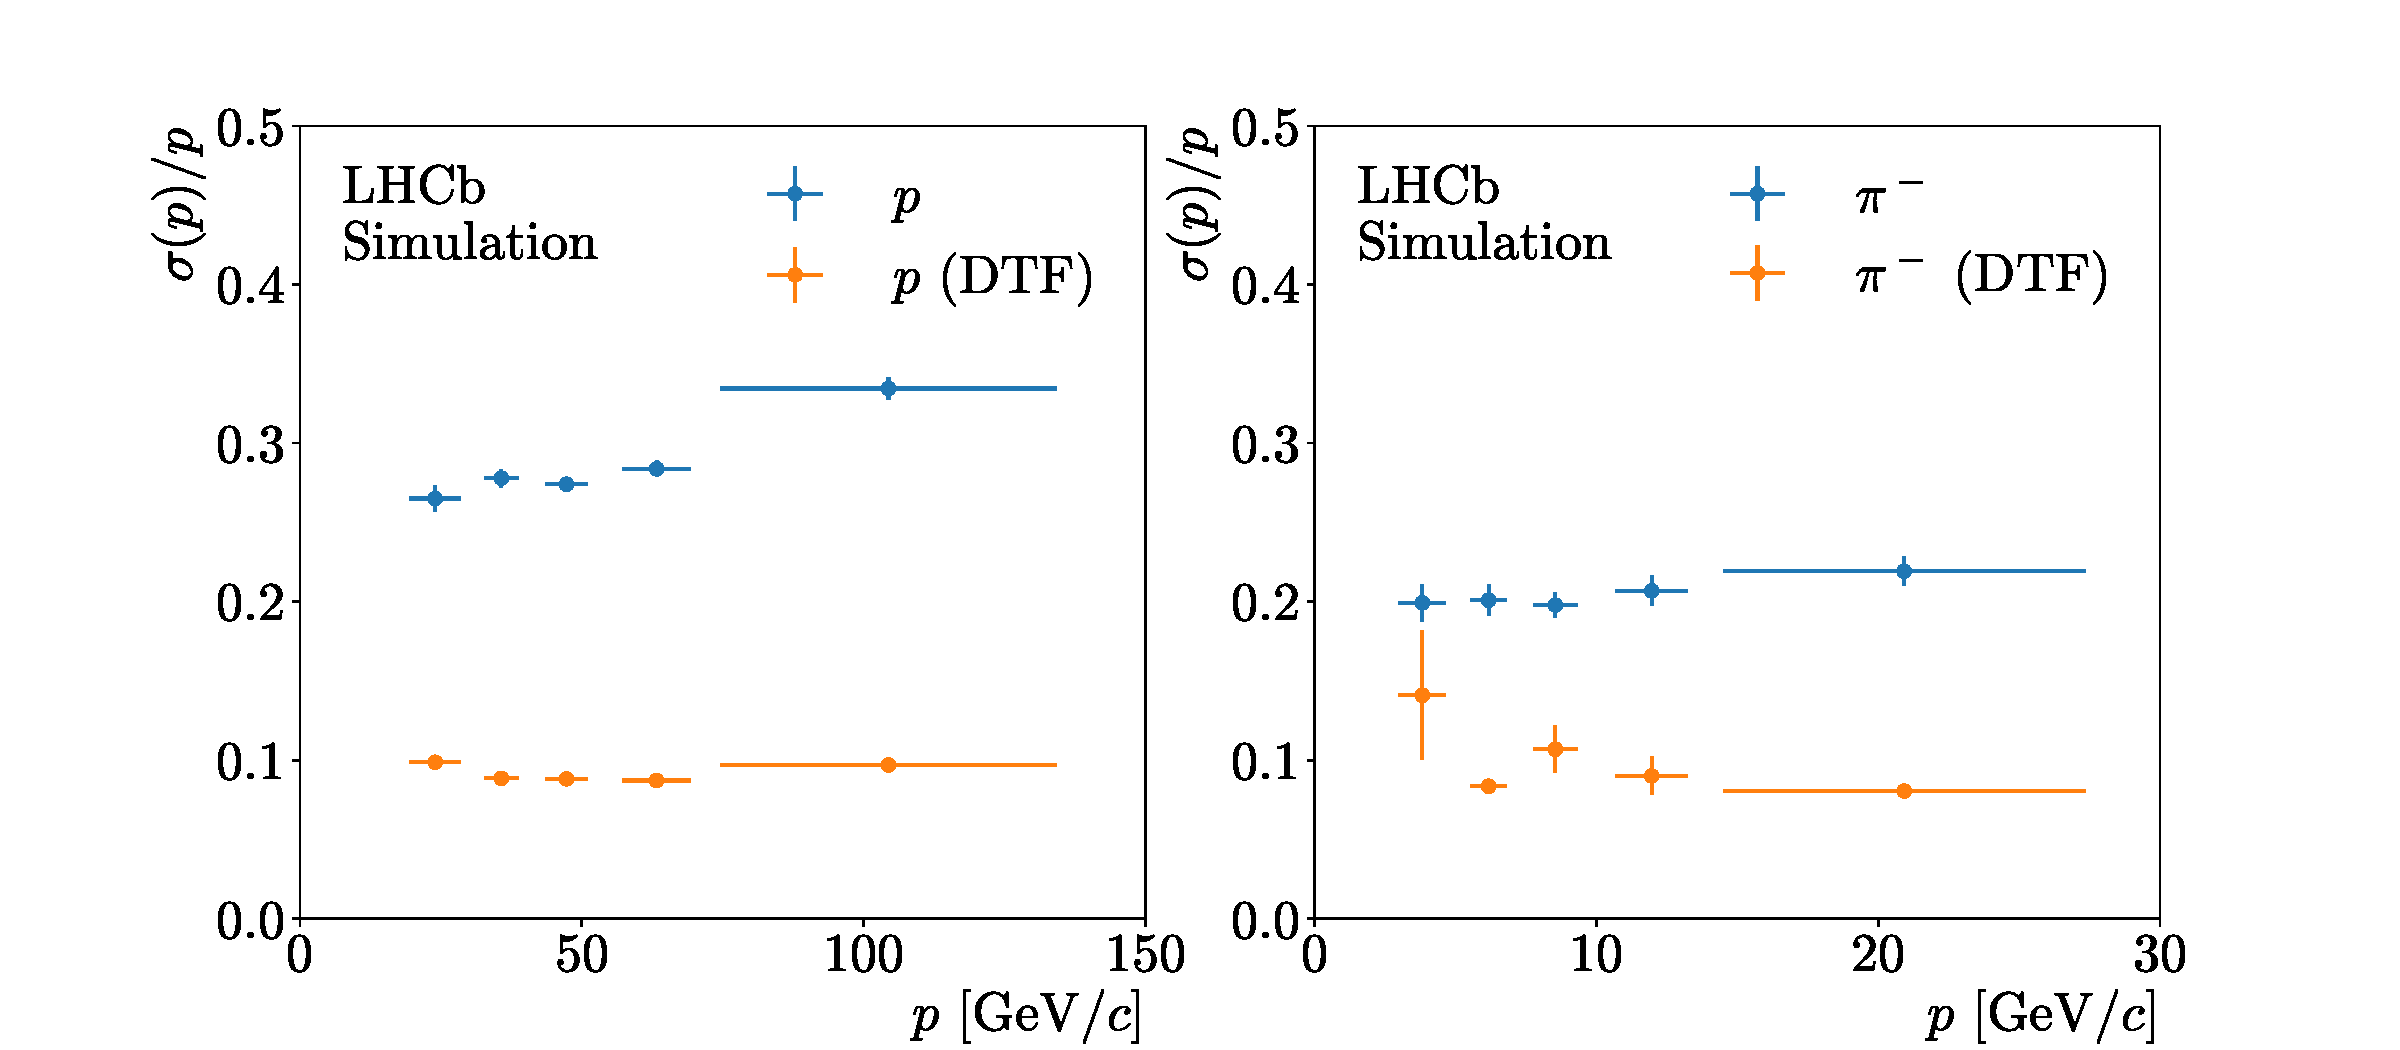
\includegraphics[width=\textwidth]{graphics/04-event_selection/paper_momentum_resolutions.pdf}
	\caption[Momentum resolution.]{Momentum resolution.}
	\label{fig:paper_momentum_resolutions}
\end{figure}

While this step introduces another filtering process and related efficiency to account for\footnote{DTF convergence efficiency with the double mass constraint is relatively uneven across the $z_\Lambda^\textbf{vtx}$ spectrum, starting at $\approx 50\%$ for $z_\Lambda^\textbf{vtx} \approx \SI{6}{\meter}$ and growing up to $\approx 85\%$ for $z_\Lambda^\textbf{vtx} \approx \SI{7.5}{\meter}$.
Comparatively, vertex reconstruction is still the primary cause of event loss in this analysis.}, it proves invaluable for our physics motivations as it mitigates the most problematic drawback of T track usage, momentum resolution.
As shown in Figure \ref{fig:paper_momentum_resolutions}, using both \jpsi and \lz mass constraints improves $\vec{p}$ resolution from $20$--$30\%$\footnote{Pion momentum resolution is higher because the pion receives a smaller fraction of the \lz momentum, thereby having a larger bending curve than the proton and allowing for better momentum measurement at the T stations.} to $\approx 10\%$.

%% Con KineAtVtx non è più vero.
%For the purposes of the helicity angle analysis outlined in Section \ref{sec:lambda}, particle momenta computed with the DTF algorithm are particularly valuable because, in addition to their greater accuracy, they are provided directly at the production vertex;
%by contrast, VF momenta are provided either at the decay vertex (short-lived particles) or at the position of first measurement (long-lived or stable particles).

\section{Reconstruction efficiency of the \texorpdfstring{$\Lambda^0_b$}{Lambdab} and \texorpdfstring{\lz}{Lambda} decays}
\label{sec:reco_efficiency}

To compute the vertex reconstruction efficiency for the \lbz decay chain, it is useful to conceptualize our event selection as a five step process:
\begin{enumerate}
	\item reconstruction of associated tracks for all charged daughter particles;
	\item reconstruction of the three decay vertices (\lz, \jpsi and \lbz);
	\item preliminary selections based on kinematic variables to filter out most background (see Section \ref{sec:prefilter});
	\item Decay Tree Fitter refit with appropriate mass constraints for the analysis at hand (usually \jpsi and \lz);
	\item further selections applied to events passing all previous steps. Detailed in Chapter \ref{cap:event_selection}, these include a physical background veto and signal selection via a trained multivariate classifier.
\end{enumerate}

For the purposes of this section, we are interested in the first two steps (track and vertex reconstruction).

Efficiencies are computed with respect to \textit{reconstructible} particles, a flag attributed during the simulation process based on the number of \textit{hits} (charged clusters with defined positions) in specific modules of the LHCb detector.
A track is said to be reconstructible as VELO track with hits in $\geq 3$ VELO modules, while it's reconstructible as T track with $\geq 1$ hits in both the $x$ and stereo layers of each T station.
If these conditions are satisfied simultaneously, the track qualifies for reconstructibility as Long track \cite{Li:2752971}.

At Monte Carlo level, a track is deemed to be \textit{reconstructed} if it can be successfully matched to at least one MC particle;
for T and Long tracks, this is true if at least $70\%$ of the hits from the respective relevant detectors for reconstructibility are shared between reconstructed and true track. For $\Lambda^0_b$ events with a true $z_\text{vtx}^\Lambda \in [\SI{6.0}{\meter}, \SI{7.6}{\meter}]$, this results in a track reconstruction efficiency in the 60\% to 80\% range.

\begin{figure}[t!]
	\centering
	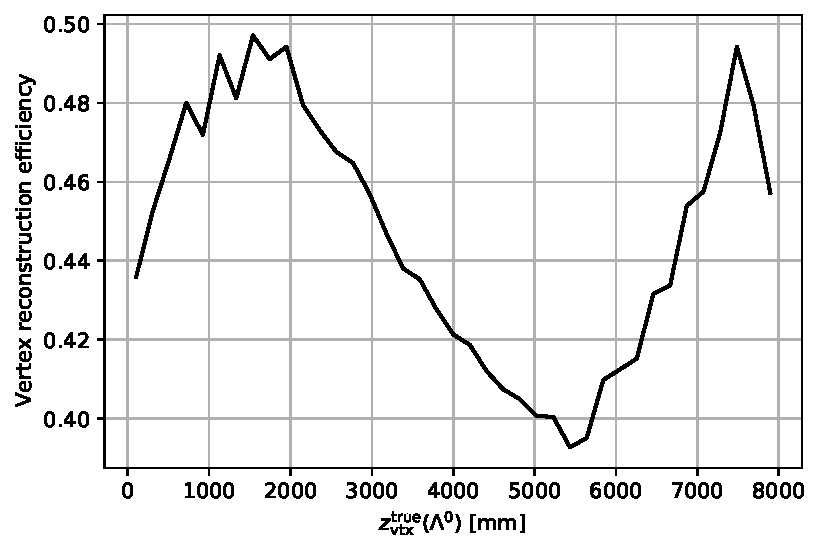
\includegraphics[width=.6\textwidth]{graphics/03-vertex_reconstruction/lambda_lambdab_reco_efficiency.pdf}
	\caption[A]{Reconstruction efficiency of simulated $\Lambda^0_b \rightarrow J/\psi~(\rightarrow \mu^+\mu^-)~\Lambda^0~(\rightarrow p\pi^-)$ events as function of the $z$ component of the true \lz decay vertex. Given that $J/\psi \rightarrow \mu^+ \mu^-$ events are reconstructed as part of the trigger step, the low efficiency is attributed to failure in reconstructing \lz and \lbz decay vertices.}
	\label{fig:lambda_lambdab_reco_efficiency}
\end{figure}

When considering how many of these reconstructed charged particles pass the vertex reconstruction (\textit{vertexing}) process, the computed efficiency is much lower.
Figure \ref{fig:lambda_lambdab_reco_efficiency} plots the resulting \lbz vertexing efficiency through the whole true $z_\text{vtx}^\Lambda$ spectrum, showing that said efficiency never manages to get past the 50\% threshold.
This means that over half of our candidate signal events is lost during the second step of the five step selection process.

While available information does not distinguish between the three individual vertexing phases (\jpsi, \lz and \lbz), we can make some reasonable assumptions.
Being Long tracks, muons and antimuons have well reconstructed momentum with constraints across the LHCb detector;
for this reason their influence on the vertexing efficiency dip is considered negligible.
Furthermore, the rare usage of T tracks for physics analysis in LHCb suggests that problems are likelier to arise in the $\Lambda^0 \rightarrow p\pi^-$ vertexing and then cascade into the $\Lambda_b^0 \rightarrow J/\psi\,\Lambda^0$ reconstruction.

For the above reasons, in the following sections I'll focus on the $\Lambda^0 \rightarrow p\pi^-$ decay to search for issues and solutions, with the goal of improving signal yield.


\section{Characterization of non-converged events}
\label{sec:characterization_non_converged}

[@todo]

The full simulated \demonstratorshort dataset constructed for studies on the measurement of the \lz electromagnetic dipole moments omits a lot of technical information on the decays, the retention of which would make storage and quick access impractical.
Furthermore, a lot of the work in this and the next sections required direct changes to the vertexing algorithm for debugging and event recovery, which in turn required data to be reprocessed.
For these reasons, the studies in the following sections were conducted on a smaller sample of [@todo:how\_many] \lbz decays.

\subsection{Behaviour through VF iterations}
\label{sec:oscillation}
The VF process reaches convergence if either condition \eqref{eq:cond_conv_1} or \eqref{eq:cond_conv_2} is satisfied, i.e. if the vertex position estimated at iteration $i$ and the one from iteration $i-1$ are <<close enough>> either in absolute distance or $\chi^2$ distance, up until $i_\text{max} = 10$.
This is predicated on the principle that the algorithm refines its vertex estimate after each iteration, homing in on the candidate vertex with the lowest $\tilde{\chi}^2_\text{vtx}$.

Such a behaviour is not found in non-converging (henceforth also known as \textit{failed}) events.
This can be seen by increasing $i_\text{max}=100$, which causes a negligible $\approx 2\%$ increase in converged events.
It follows that, for the vast majority of missing events, failure of convergence is not a product of low computation time and must instead result from some internal malfunction of the vertexing process.

\begin{figure}[t]
	\centering
	\begin{subfigure}{.45\textwidth}
		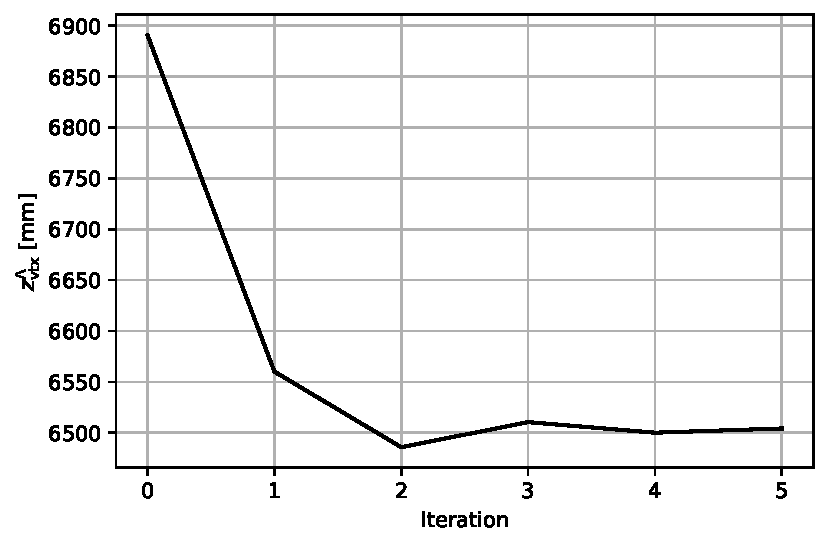
\includegraphics[width=\textwidth]{graphics/03-vertex_reconstruction/evt0_vertex_z.pdf}
		\caption{}
		\label{fig:z_iter_conv}
	\end{subfigure}
	\begin{subfigure}{.45\textwidth}
		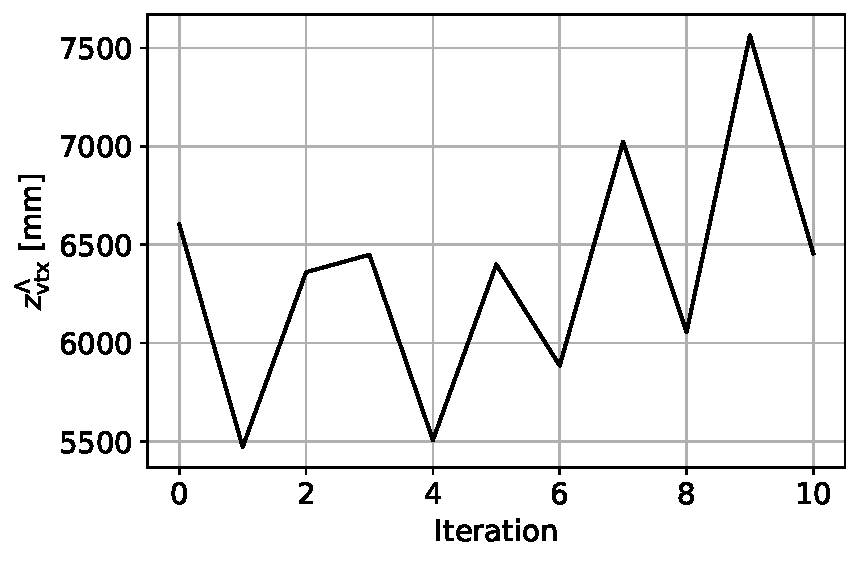
\includegraphics[width=\textwidth]{graphics/03-vertex_reconstruction/evt83_vertex_z.pdf}
		\caption{}
		\label{fig:z_iter_failed}
	\end{subfigure}
	\caption{Best values of tentative \lambdadecay vertex $z$ component at the end of each Vertex Fitter iteration for examples of converged \textit{(a)} and failed \textit{(b)} events.}
	\label{fig:z_iter_conv_vs_failed}
\end{figure}

This is readily apparent when studying the vertex positions throughout the iterating process for examples of converged and failed events of simulated signal.
Figure \ref{fig:z_iter_conv_vs_failed} compares the values of $z_\text{vtx}^\Lambda$, the $z$ component of the \lambdadecay decay vertex, as reconstructed by the VF in iterations $i=0$ to $10$ ($i=0$ being the starting seed).
Figure \ref{fig:z_iter_conv} (converged) exhibits the expected behaviour, with the algorithm refining its vertex estimate after every iteration and finally converging as early as $i=5$.
By contrast, Figure \ref{fig:z_iter_failed} (failed) presents an \textit{oscillating behaviour} of $z_\text{vtx}^\Lambda$, swinging by as much as \SI{1}{\meter} in the opposite direction after an iteration completes.
While a particularly tricky instance of the first type of event may potentially benefit by an increased $i_\text{max}$, no amount of allotted computations can lead the second type to convergence.

\begin{figure}[t]
	\centering
	\begin{subfigure}{.45\textwidth}
		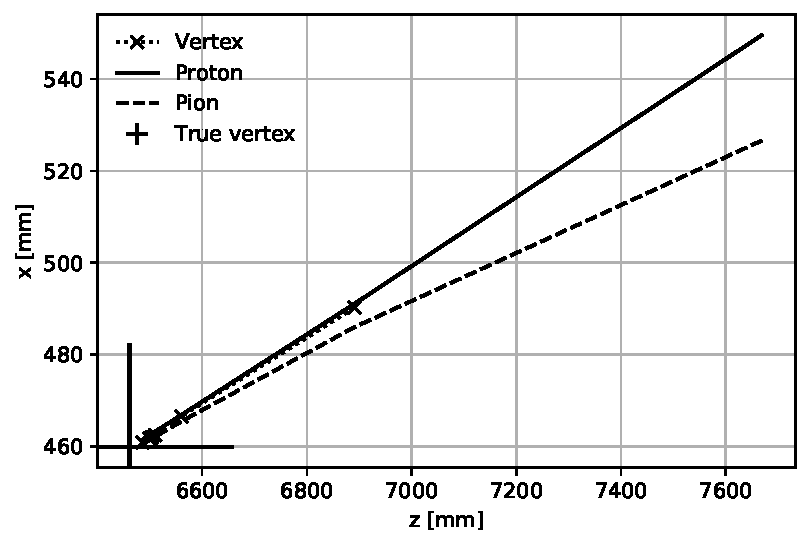
\includegraphics[width=\textwidth]{graphics/03-vertex_reconstruction/evt_0_zx.pdf}
		\caption{}
		\label{fig:3:converged_zx}
	\end{subfigure}
	\begin{subfigure}{.45\textwidth}
		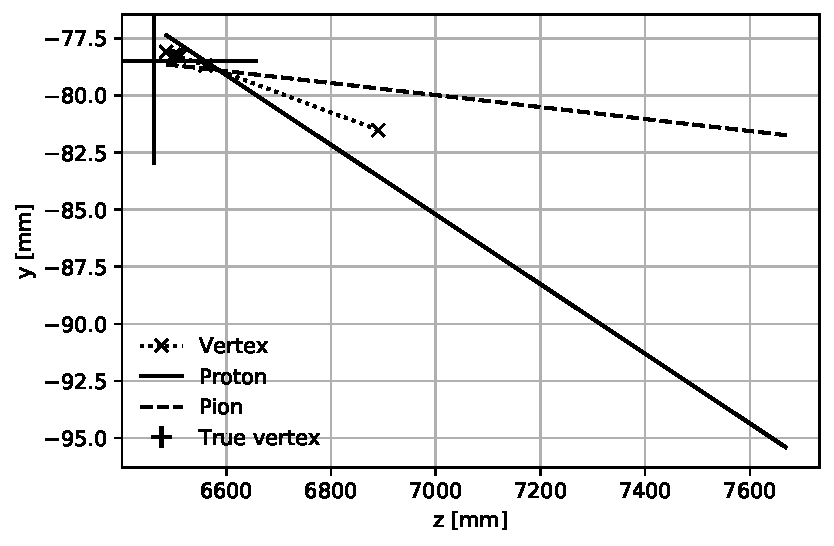
\includegraphics[width=\textwidth]{graphics/03-vertex_reconstruction/evt_0_zy.pdf}
		\caption{}
		\label{fig:3:converged_zy}
	\end{subfigure}
	\caption{\lambdadecay decay topology for an instance of converged event, projected in the $xz$ \textit{(a)} and $yz$ \textit{(b)} planes.
	The temporary best vertex locations chosen by the Vertex Fitter at the end of each iterations are marked with \textit{diagonal crosses} and linked by the \textit{dotted line} in iteration order (the second iteration best vertex is connected to the first, the third to the second and so on).
	The reconstructed vertex, while not explicitly represented, can be identified by the cluster of vertex point markers.
	At the beginning of each iteration, daughter particles are extrapolated at the $z$ of the best vertex of the previous iteration: proton (\textit{solid line}) and pion (\textit{dashed line}) tracks are drawn joining the respective reference points after transportation in order of decreasing $z$ (i.e. not in iteration order).
	The true vertex is marked by the \textit{large Greek cross}.}
	\label{fig:3:converged_event_topology}
\end{figure}

We can gain more insight into the nature of this oscillation by approaching the problem from a more <<geometrical>> point of view.
Figure \ref{fig:3:converged_event_topology} shows the topology of the converged event from Figure \ref{fig:z_iter_conv} in the bending $xz$ and non-bending $yz$ planes.
While the points of closest distance between the tracks in the two planes are not exactly matched, the algorithm manages to converge on a vertex position that is reasonably close to the true position from the generated decay.

\begin{figure}[t]
	\centering
	\begin{subfigure}{.45\textwidth}
		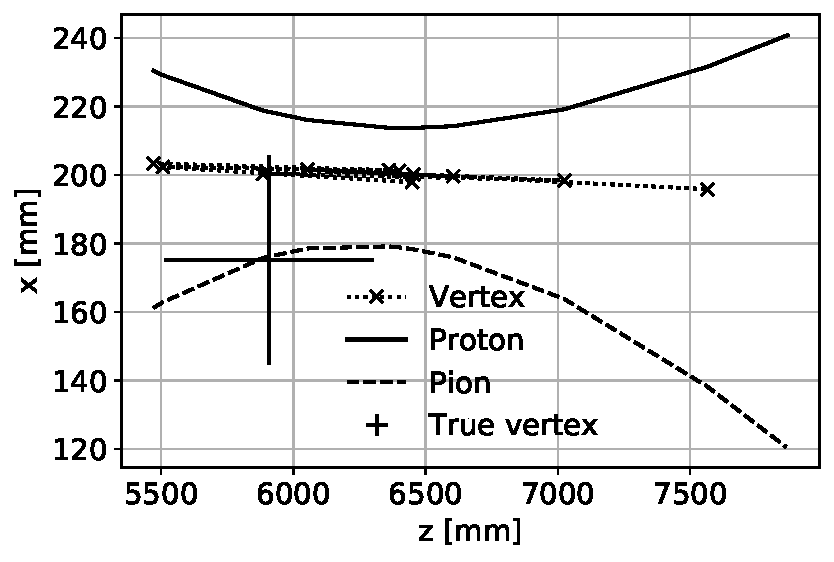
\includegraphics[width=\textwidth]{graphics/03-vertex_reconstruction/evt_83_zx.pdf}
		\caption{}
		\label{fig:3:failed_zx}
	\end{subfigure}
	\begin{subfigure}{.45\textwidth}
		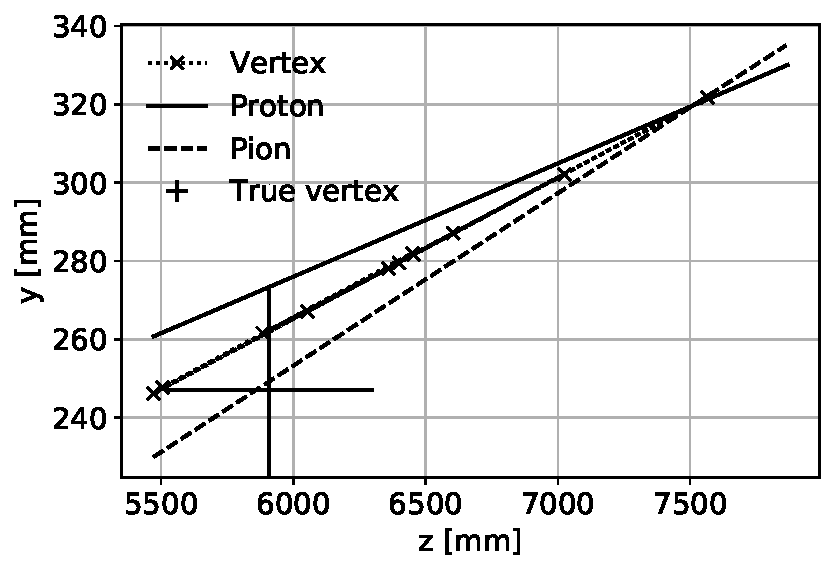
\includegraphics[width=\textwidth]{graphics/03-vertex_reconstruction/evt_83_zy.pdf}
		\caption{}
		\label{fig:3:failed_zy}
	\end{subfigure}
	\caption{\lambdadecay decay topology for an instance of non-converged event, projected in the $xz$ \textit{(a)} and $yz$ \textit{(b)} planes.
	Notation follows the one in Figure \ref{fig:3:converged_event_topology}.}
	\label{fig:3:failed_event_topology}
\end{figure}

The behaviour for the non-converged event from Figure \ref{fig:z_iter_failed}, shown in Figure \ref{fig:3:failed_event_topology}, is drastically different.
The dotted line following the best vertex estimate through iterations in the bending plane (Figure \ref{fig:3:failed_zx}) shows that the algorithm gravitates \textit{around} the point of closest distance between proton and pion tracks ($z \approx \SI{6.25}{\meter}$), never outright choosing it as candidate.
On the other hand, in the $yz$ plane (Figure \ref{fig:3:failed_zx}) the two tracks cross at a much more downstream point ($z \approx \SI{7.5}{\meter}$), which the Vertex Fitter also largely ignores during the iteration process.

%Some more insight into the nature of this oscillation can be achieved by taking a more <<geometrical>> look, plotting inter-iteration vertex coordinates in the $zx$ plane where the LHCb magnet bends tracks according to their charge.
%Figure \ref{fig:zx_iter_conv_vs_failed} compares the same events from Figure \ref{fig:z_iter_conv_vs_failed}.
%Again, the converged event in Figure \ref{fig:zx_iter_conv} behaves as intended, selecting as vertex roughly the point of closest distance between the tracks (some leeway is accorded since the fit also incorporates information from $xy$ and $yz$ planes).
%The progress in Figure \ref{fig:zx_iter_failed} is more interesting: in the failed case the estimated vertex, identified at each iteration by <<x>> markers along the dashed line, appears to gravitate \textit{around} the point of closest distance, never outright choosing it as candidate.
%Significantly, the \textit{true} $\Lambda^0$ vertex (marked by the green cross) lags some \SI{50}{\centi\meter} behind it.


\begin{figure}[t]
	\centering
	\begin{subfigure}{.45\textwidth}
		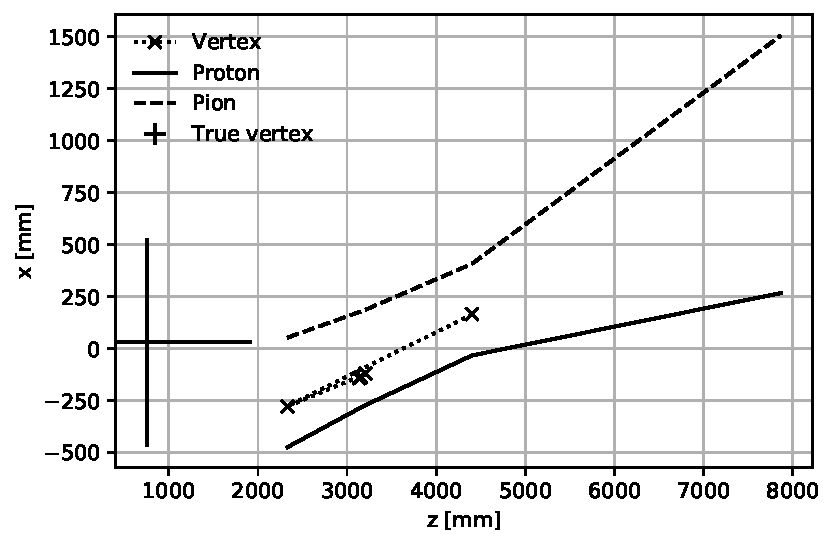
\includegraphics[width=\textwidth]{graphics/03-vertex_reconstruction/evt_6_zx.pdf}
		\caption{}
		\label{fig:3:converged_detached_zx}
	\end{subfigure}
	\begin{subfigure}{.45\textwidth}
		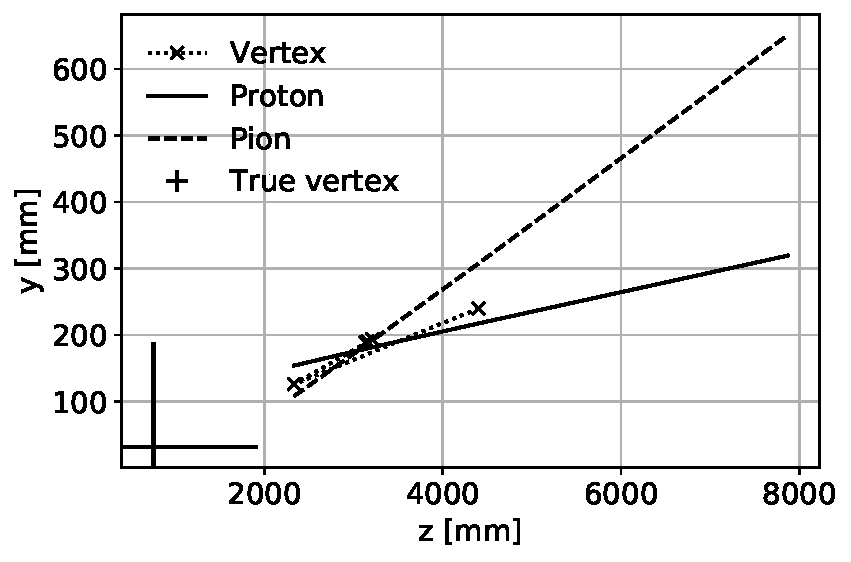
\includegraphics[width=\textwidth]{graphics/03-vertex_reconstruction/evt_6_zy.pdf}
		\caption{}
		\label{fig:3:converged_detached_zy}
	\end{subfigure}
	\caption{\lambdadecay decay topology for an instance of converged event with large track gap in the $xz$ plane, projected in the $xz$ \textit{(a)} and $yz$ \textit{(b)} planes.
	Notation follows the one in Figure \ref{fig:3:converged_event_topology}.}
	\label{fig:3:converged_detached_event_topology}
\end{figure}

It may be tempting to attribute the failed convergence in this event to the comparatively larger gap between proton and pion tracks at their point of closest distance in the bending plane.
However, the VF algorithm has shown to be capable of bridging an imperfect track extrapolation: the converged event shown in Figure \ref{fig:3:converged_detached_event_topology} has a closest track distance of some \SI{40}{\centi\meter}, an order of magnitude greater than the track distance seen in Figure \ref{fig:3:failed_event_topology}.
Despite the large gap, the VF is able to recognize $z \approx \SI{3}{\meter}$ as the best candidate for the vertex, even if said point is far removed from the actual \lambdadecay decay vertex.

%While it may be tempting to attribute the failed convergence to the comparatively larger gap between proton and pion tracks at their point of closest distance, some observations are in order:
%first, the deceivingly different $x$ scales in Figures \ref{fig:zx_iter_conv} and \ref{fig:zx_iter_failed} mean that in the latter tracks are closer than they may seem;
%more to the point, the VF algorithm has shown to be capable of bridging an imperfect track extrapolation in converged events, as demonstrated in Figure \ref{fig:zx_iter_conv_backstep}.



%%%%%%%%%%%%%%%%%%%%%%%%%%%%%%%%%%%%%%%%%%%%%%%%%%%%%%%%%%%%%%%%%%%
a
%%%%%%%%%%%%%%%%%%%%%%%%%%%%%%%%%%%%%%%%%%%%%%%%%%%%%%%%%%%%%%%%%%%

We can make a more convincing remark by analyzing performance in the $yz$ plane, where tracks \textit{don't} bend.
Figure \ref{fig:zy_iter_conv} shows that, in the converged case, the $yz$ track crossing is $z$-aligned with the closest $xz$ distance point.
This doesn't happen for the failed event: while Figure \ref{fig:zy_iter_failed} shows that $yz$ tracks cross almost coinciding with the true vertex position, we have already pointed out that this is \SI{50}{cm} short of the $xz$ closest distance point.
Convergence failure for the event in Figures \ref{fig:zx_iter_failed} and \ref{fig:zy_iter_failed} can thus be interpreted through the lens of \textit{conflicting information}:
the best vertex candidate has different $z_\text{vtx}$ in the $xz$ (with magnetic field) and $yz$ (without magnetic field) planes, and the VF algorithm flip-flops between the two.

For didactic purpose, the analysis in this section has focused on just one event.
All the emerged patterns are however commonplace throughout the failed events I have examined, with the oscillating vertex behaviour in particular being a constant in almost all of them.
While every \lbz vertexing failure being the fault of $xz$ and $yz$ track mismatch would be a reckless conclusion, I have been able to use these findings, along with other from the following paragraphs, to devise a partial solution in Section \ref{sec:blowup_matrix}.

%\subsection{True kinematics}
%To further investigate the possible source of the oscillating behaviour outlined in Section \ref{sec:oscillation}, I have conducted a systematic comparison of kinematic features at Monte Carlo level between converged and failed events.
%
%No difference among the two categories emerge when considering basic decay descriptors such as the momenta of all particles involved and the decay vertices of unstable particles.
%Moreover, there doesn't seem to be a critical decay geometry that triggers the vertexing;
%for instance, there is no evidence that $\Lambda^0 \rightarrow p\pi^-$ decays lying largely in the $xz$ plane, a setup quite unfriendly to the VF algorithm (see Section \ref{sec:lambda_endvertex_bias}), has any disproportionate representation amongst non-converged events.
%
%\subsection{Kinematics at first measurement position}
%\label{sec:3:kinematics_at_first_meas}
%A major discrepancy emerges when looking at particle interaction with the detector via \textit{protoparticles}.
%A protoparticle is a data structure created during the LHCb event reconstruction process with the intent of encapsulating all relevant information available for the associated particle:
%particle identification (PID) from the RICH and muon detectors, results from calorimeter hits and track information.
%The latter contains details on momentum in relation to a certain reference point which, for stable charged particles, corresponds to the position of first measurement.
%
%\begin{figure}[t]
%	\centering
%	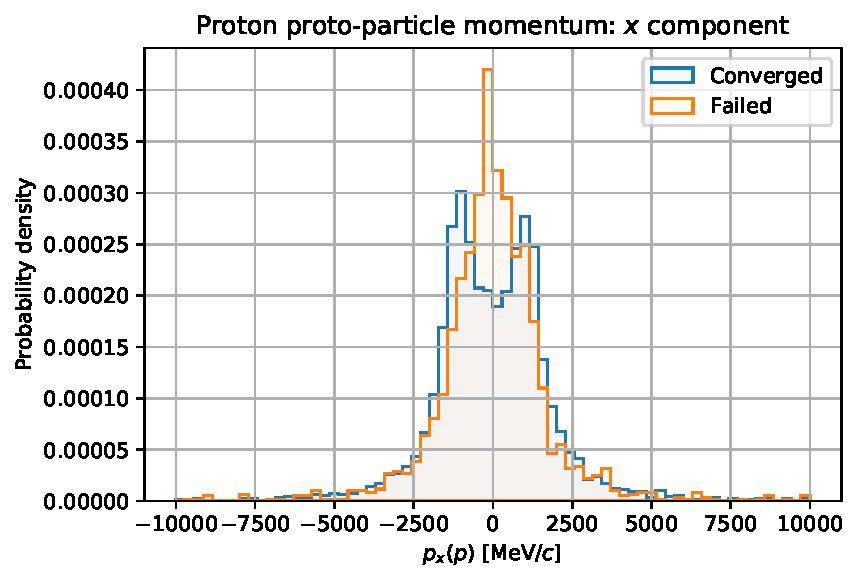
\includegraphics[width=.6\textwidth]{graphics/03-vertex_reconstruction/pp_p_momentum_x.pdf}
%	\caption{A.}
%	\label{fig:pp_p_px_conv_vs_failed}
%\end{figure}
%
%In the case of simulated protons from $\Lambda_b^0 \rightarrow J/\psi\,\Lambda^0$ decays, the distribution of the
%%true\footnote{While protoparticles result from interaction of the particle with the material, at this point I'm specifically considering the true value of the first measurement position and related momentum. Later on we'll instead delve into the \textit{reconstructed} counterparts of these quantities, which can be different as a result of poor T station measurements.}
%protoparticle $p_x$ for converged and failed events shows a marked difference outlined in Figure \ref{fig:pp_p_px_conv_vs_failed}:
%correctly reconstructed events tend to have a double peak roughly centered in $\approx \pm \SI{1}{\gev}$, while missing events have a more traditional single peak centered in $0$.
%
%%% todo: spezza in due? Fixa anche il testo poco dopo.
%\begin{figure}[t]
%	\centering
%	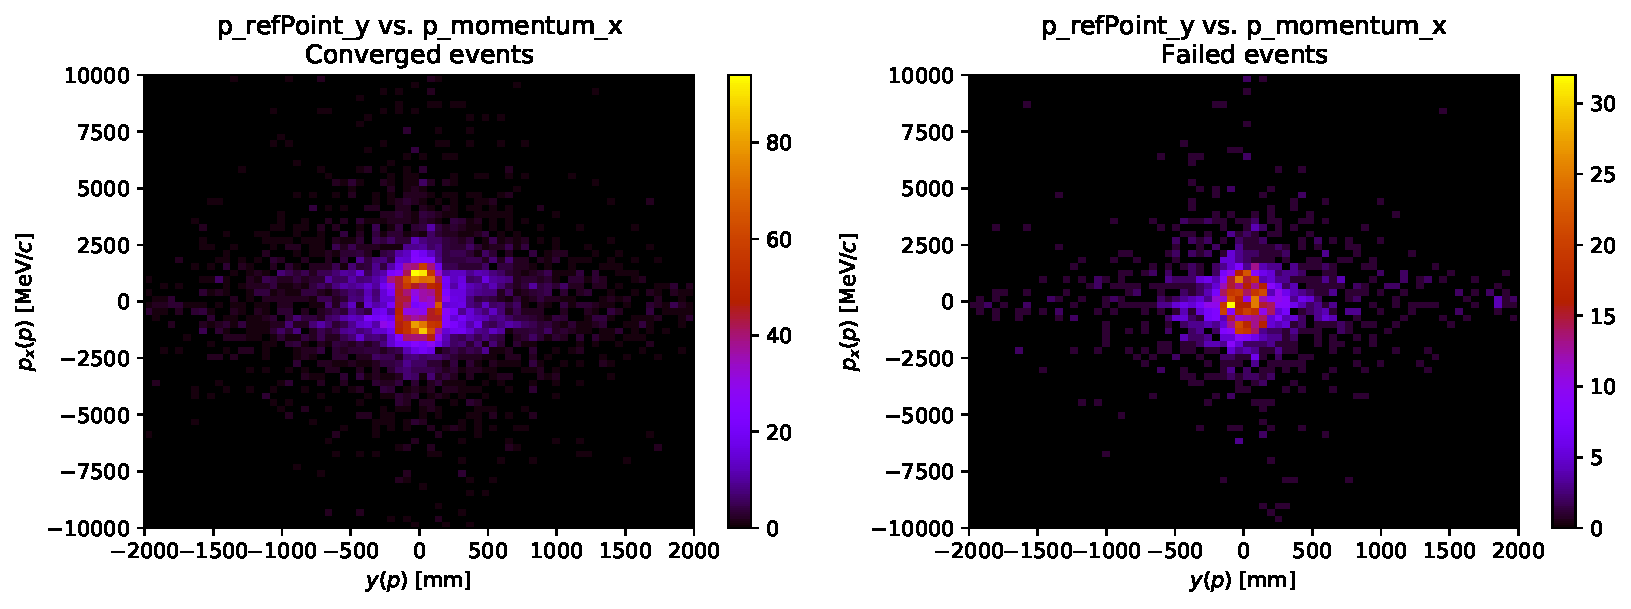
\includegraphics[width=\textwidth]{graphics/03-vertex_reconstruction/pp_p_refPoint_y_vs_p_momentum_x.pdf}
%	\caption{B.}
%	\label{fig:pp_p_px_vs_refpy_conv_vs_failed}
%\end{figure}
%
%Even more interestingly, this discrepancy can be put in relation to the $y$ component of the protoparticle first measurement position, as seen in Figure \ref{fig:pp_p_px_vs_refpy_conv_vs_failed}.
%The ring-like structure in Figure \ref{fig:pp_p_px_vs_refpy_conv_vs_failed} implies that the vertexing process struggles to reconstruct proton protoparticles with low $p_x$ hitting the T stations at $y\approx 0$.
%No such discrepancy is present in the case of pions.
%
%A precise estimate of $p_x$ is of paramount importance for correct track measurement and extrapolation.
%Even slight mistakes in angle assessment are magnified during particle transportation through long distances, especially since the T track requirement leaves no upstream constraints.
%Moreover, momentum itself is computed through evaluation of the particle bending curve in the $xz$ plane induced by the magnet.
%As such, it stands to reason that poor measurement of the low proton $p_x$ can have enough of an effect to throw off the vertexing algorithm.


%%%%%%%%%%%%%%%%%%%%%%%%%%%%%%%%%%%%%%%%%%%%%%%%%%%%%%%%%%%%%

\subsection{Study of decay kinematics before and after interaction with the detector}
\label{sec:3:kinematics_at_first_meas}
To gather information on the possible sources of the oscillating behaviour outlined in Section \ref{sec:oscillation}, I investigated the collective properties of a sample of \demonstratorshort decays in search of significant discrepancies between converged and failed events.

No difference between the two categories emerged at Monte Carlo level when considering the true values of basic kinematic variables such as daughter particle momenta or decay vertices locations of the three unstable particles \lbz, \lz and \jpsi.
Moreover, there doesn't seem to be a critical decay geometry that triggers the vertexing issues;
for instance, there is no evidence that \lambdadecay decays lying largely in the $xz$ plane, a setup quite unfriendly to the VF algorithm (see Section \ref{sec:lambda_endvertex_bias}), have any disproportionate representation amongst non-converged events.
This rules out the hypothesis that the failure of vertex fit convergence be caused by particle characteristics at production, such as protons and pions with unusually low transverse momentum \pt.

I also considered the possibility that kinematic asymmetries between converged and failed events may arise after interaction with the LHCb detector;
one example of this would be the case where failed events correlate with hits in a specific sections of the IT or OT trackers.
To this end I studied the event \textit{protoparticles}, data structures created during the LHCb event reconstruction process with the intent of encapsulating all relevant information available for the associated particle:
particle identification from the RICH and muon detectors, results from calorimeter hits and track information.
Tracks themselves contain details on momentum in relation to a certain reference point which, for stable charged particles, corresponds to the position of first measurement.

\begin{figure}[t]
	\centering
	\begin{subfigure}{.45\textwidth}
		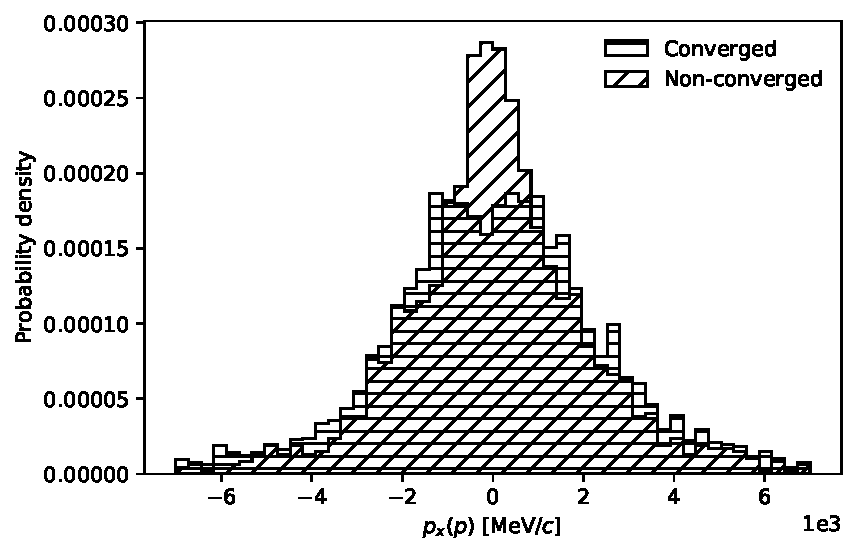
\includegraphics[width=\textwidth]{graphics/03-vertex_reconstruction/p_momentum_x.pdf}
		\caption{}
		\label{fig:3:p_momentum_x}
	\end{subfigure}
	\begin{subfigure}{.45\textwidth}
		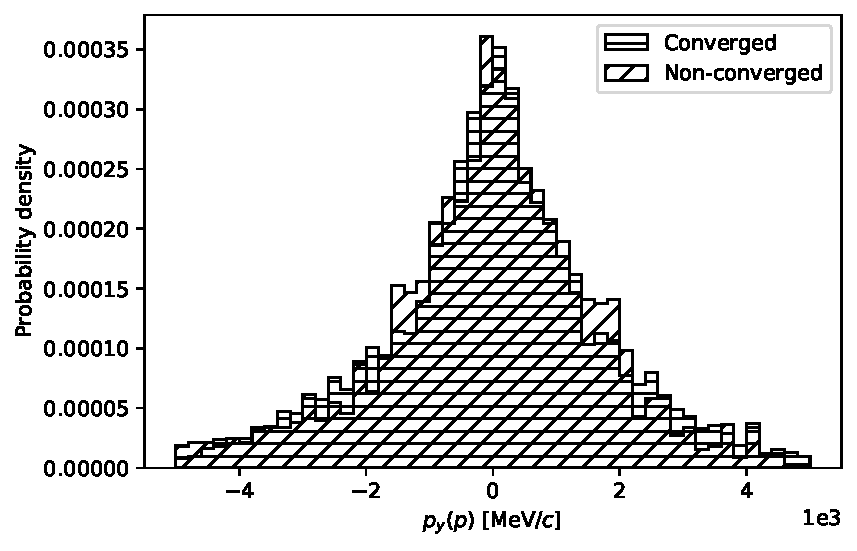
\includegraphics[width=\textwidth]{graphics/03-vertex_reconstruction/p_momentum_y.pdf}
		\caption{}
		\label{fig:3:p_momentum_y}
	\end{subfigure}
	\caption{Normalized distributions of proton protoparticles $p_x$ \textit{(a)} and $p_y$ \textit{(b)} components. Distributions of events with converging vertex are depicted with \textit{horizontal hatching}, non-converging with \textit{diagonal hatching}.}
	\label{fig:3:p_protioparticle_momenta}
\end{figure}

Figure \ref{fig:3:p_momentum_x} depicts the only major discrepancy between converged and failed events I found in this process:
non-converged \lbz decays have a proton protoparticle $p_x$ distribution concentrated in $p_x \approx 0$, while converged decays show even dispersion of the central peak in the $[-\SI{1}{\gev},\SI{1}{\gev}]$ region.
This is to be contrasted with $p_y$, the other component of the protoparticle transverse momentum, whose two distributions are almost overlapping (Figure \ref{fig:3:p_momentum_y}).
While statistics in the reduced samples are too low to say for sure, pions do not appear to show similar discrepancies in their protoparticles.

Assuming $p_x$ measurement at detector level is not biased, this result suggests that protons from failed events have generally lower $p_x$ when they reach the T stations;
this would not be apparent from \pt distributions at the point of production, since the final $p_x$ value depends on the bending radius imprinted by the magnet (which in turn depends on momentum and distance traveled).
Such low values of $p_x$ are potentially more susceptible to poor measurement by the T stations, which in turn affects the overall momentum resolution based on the particle bending radius in the $xz$ plane.

%Low values of $p_x$ imply roughly perpendicular incidence in the $xz$ bending plane used for momentum measurement by the T stations, which would affect the already poor momentum resolution 
%
%The correlation between low proton protoparticle $p_x$ and vertexing failure contains a valuable hint:
%converged and failed events may not differ in \pt of protons and pions at the point of productions, but it's possible that they do at the point of first measurement, after the particles are bent by the magnet.
%
%Poor measurement of $p_x$
%
%A precise estimate of $p_x$ is of paramount importance for correct track measurement and extrapolation:
%even slight mistakes in angle assessment are magnified during particle transportation through long distances, especially since the T track requirement leaves no upstream constraints.
%Moreover, momentum itself is computed through evaluation of the particle bending curve in the $xz$ plane induced by the magnet.
%As such, \lambdadecay events with low $p_x (p)$ when the proton reaches the T stations would be more suscetible to poor momentum measurement and 
%
%The link between 
%
%
%As such, one possible interpretation of the correlation between proton protoparticle $p_x$ and failure in vertexing is that 
%One possible interpretation is thus that
%
%As such, it stands to reason that poor measurement of the low proton $p_x$ can have enough of an effect to throw off the vertexing algorithm.

\subsection{Study of decay kinematics after extrapolation}
\label{sec:3:true_vtx_kinematics}
As will be later discussed in Sections \ref{sec:blowup_matrix} and \ref{sec:lambda_endvertex_bias}, reconstruction of the \lz vertex is affected by a significant positive bias of median value $\mu_\frac{1}{2} \left(z_\Lambda^\text{reco} - z_\Lambda^\text{true}\right) \approx \SI{43}{\centi\meter}$.
In spite of such a discrepancy, the standard modus operandi for kinematics-at-vertex analyses usually compares the true momenta (evaluated at the true vertex) with the reconstructed momenta (evaluated at the reconstructed vertex).

For this section I have followed a different approach, instead opting to transport via Runge-Kutta extrapolator the reconstructed $p$ and $\pi^-$ at the true  $\Lambda^0 \rightarrow p\pi^-$ vertex position, injected from Monte Carlo information.
Since the extrapolator takes raw protoparticles as inputs, this process bypasses any smoothing applied during the fit process and, given an observable $f$ (particle reference points and momenta, for instance), it allows for a comparison between the true value $f_\text{true}$ and the RK-extrapolated value $f_\text{RK}$ at the actual $z_\text{vtx}^\Lambda$, circumventing the effect of vertex bias.
Any potential mismatch will be normalized in terms of \textit{residuals}
\begin{equation}
	\text{res}(f) \coloneqq \frac{f_\text{RK} - f_\text{true}}{\sigma_f^\text{RK}},
\end{equation}
with $\sigma_f^\text{RK}$ being the uncertainty computed by the RK algorithm.
Assuming a correct estimation of such uncertainties, we expect the residuals to follow a standard normal distribution.

\begin{figure}[t]
	\centering
	\begin{subfigure}{.45\textwidth}
		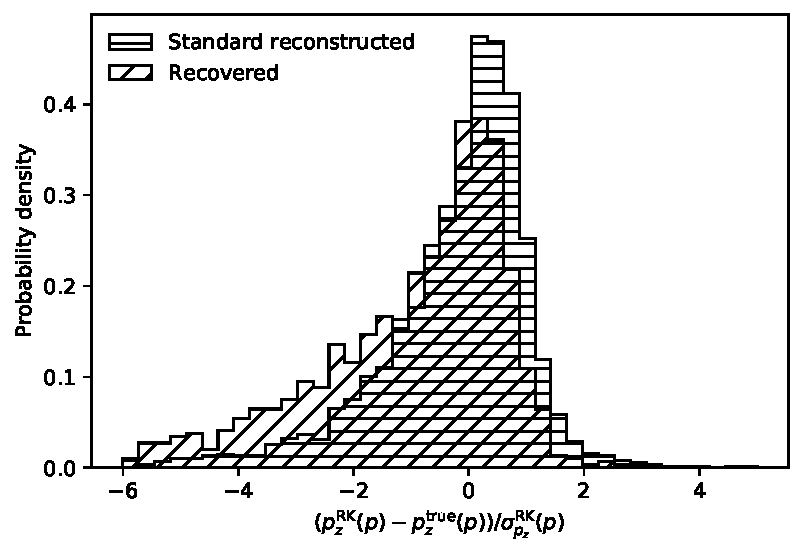
\includegraphics[width=\textwidth]{graphics/03-vertex_reconstruction/p_momentum_residual_2Dv3D_z_rel.pdf}
		\caption{}
		\label{fig:p_momentum_residual_2Dv3D_z_rel}
	\end{subfigure}
	\begin{subfigure}{.45\textwidth}
		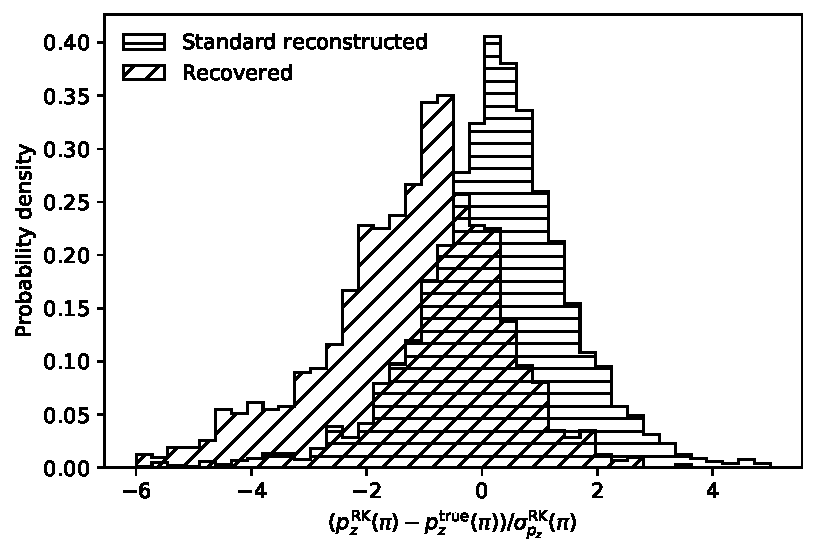
\includegraphics[width=\textwidth]{graphics/03-vertex_reconstruction/pim_momentum_residual_2Dv3D_z_rel.pdf}
		\caption{}
		\label{fig:pim_momentum_residual_2Dv3D_z_rel}
	\end{subfigure}
	\caption[A and b.]{Left right}
	\label{fig:p_pim_momentum_residual_2Dv3D_z_rel}
\end{figure}

Figure \ref{fig:p_pim_momentum_residual_2Dv3D_z_rel} shows $p_z$ residuals for proton and pions extrapolated at the \lz true decay vertex, juxtaposing converged and non-converged event distributions.
The first takeaway is that VF-reconstructed events have a remarkably non-gaussian distribution, with a slightly positive mean and asymmetric tails. 
This is particularly apparent in the case of the proton, where for $p_z^\text{RK} < p_z^\text{true}$ the RK algorithm systematically underestimates the error.
More relevant for this chapter is Figure \ref{fig:pim_momentum_residual_2Dv3D_z_rel} specifically, which highlights the fact that pion tracks from non-converged events generally sport a strong negative bias on $p_z$.

\begin{figure}[t]
	\centering
	\begin{subfigure}{.45\textwidth}
		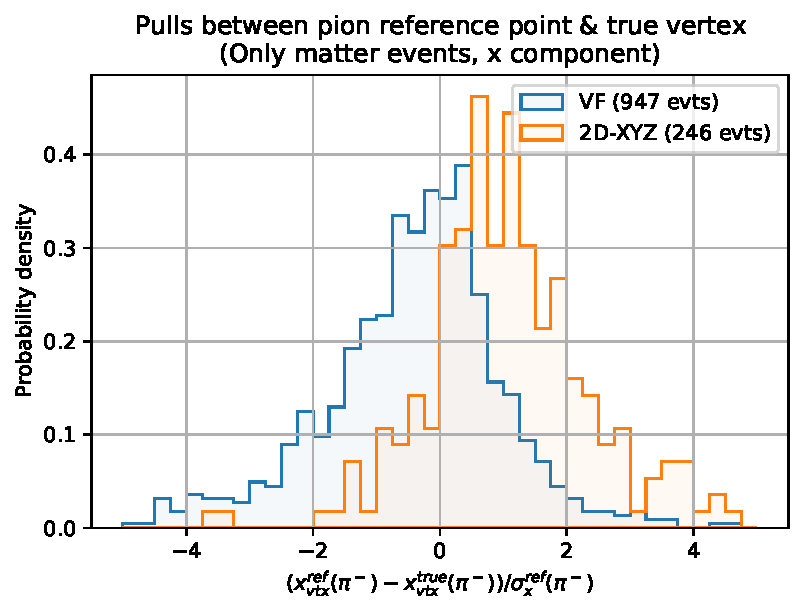
\includegraphics[width=\textwidth]{graphics/03-vertex_reconstruction/pim_refpoint_residual_2Dv3D_x_rel_matter.pdf}
		\caption{}
		\label{fig:pim_refpoint_residual_2Dv3D_x_rel_matter}
	\end{subfigure}
	\begin{subfigure}{.45\textwidth}
		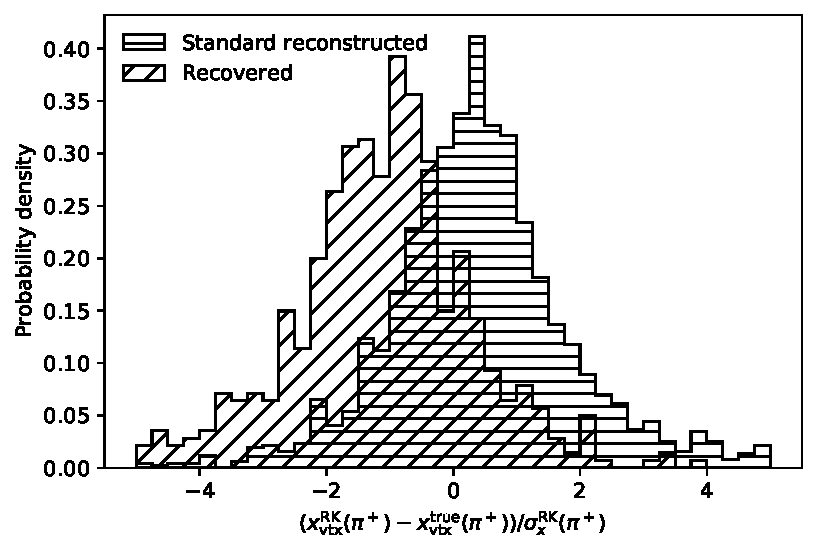
\includegraphics[width=\textwidth]{graphics/03-vertex_reconstruction/pim_refpoint_residual_2Dv3D_x_rel_antimatter.pdf}
		\caption{}
		\label{fig:pim_refpoint_residual_2Dv3D_x_rel_antimatter}
	\end{subfigure}
	\caption[A and b.]{Left right}
	\label{fig:pim_refpoint_residual_2Dv3D_x_rel}
\end{figure}

This behaviour can also be observed from a different perspective by considering the pion reference point $x$ residuals\footnote{The Runge-Kutta extrapolator transports a particle up to a specified $z$ coordinate. As a consequence, $x$ and $y$ reference points gauge the discrepancy between track extrapolation and the true position of the MC particle at said $z$, with $z_\text{ref}^\text{RK} \approx z_\text{ref}^\text{true}$ within extrapolator tolerance.}, plotted in Figure \ref{fig:pim_refpoint_residual_2Dv3D_x_rel}.
For this part of the analysis, we forgo the established omission of charge-conjugate notation and separate events in matter ($\Lambda^0 \rightarrow p\pi^-$) and antimatter ($\bar{\Lambda}^0 \rightarrow \bar{p}\pi^+$) events.
Since all events in this sample have magnet polarity $M_\text{pol} = +1$, i.e. magnetic field flowing towards the positive direction of the $y$ axis,
%% @todo: controlla che sia vero
matter and antimatter daughter particles will bend in opposite directions due to charge inversion.

Comparing Figures \ref{fig:pim_refpoint_residual_2Dv3D_x_rel_matter} and \ref{fig:pim_refpoint_residual_2Dv3D_x_rel_antimatter}, $x$ components of pion reference points in non-converged events show opposite bias when extrapolated at the \lz vertex.
Such a behaviour is easily understood in terms of transportation: tracks are extrapolated from downstream protoparticles towards decreasing $z$;
if the magnetic bending effect in the $zx$ plane is overstated (if tracks <<bend too much>>), the resulting $x$ reference point at true $z_\text{vtx}^\Lambda$ will have an offset with respect to the actual origin vertex of the particle with polarity-depdendent sign (cf. Figure \ref{fig:zx_iter_failed}).

Excessive bending is exactly what is expected of a track with correctly estimated $p_x$ and $p_y$, but underestimated $p_z$.
Furthermore, a lower $p_z$ will affect the closest distance point between proton and pions in the $zx$ plane, but will have a much lower impact on the track crossing point in the $yz$ plane,
%where bending is negligible,
supporting the conflicting information interpretation for vertex oscillation given in Section \ref{sec:oscillation}.
Considering the information gathered so far, the two most plausible causes of failed convergence appear to be wrong extrapolation by the Runge-Kutta algorithm, perhaps triggered by lower protoparticle $p_x$ observed in Section \ref{sec:3:kinematics_at_first_meas}, and/or poor measurement from T stations resulting in $p_z$ underestimation of protons and pions.

%\section{Recovery of non-converged events}
%\subsection{Recovery through refit with rescaled uncertainties}
\section[Recovery of non-converged events]{Recovery of non-converged events through refit with rescaled uncertainties}
\label{sec:recovery_general}
\label{sec:blowup_matrix}

%\subsection{Recovery through interpolation}
%@todo

%\begin{figure}[t]
%	\centering
%	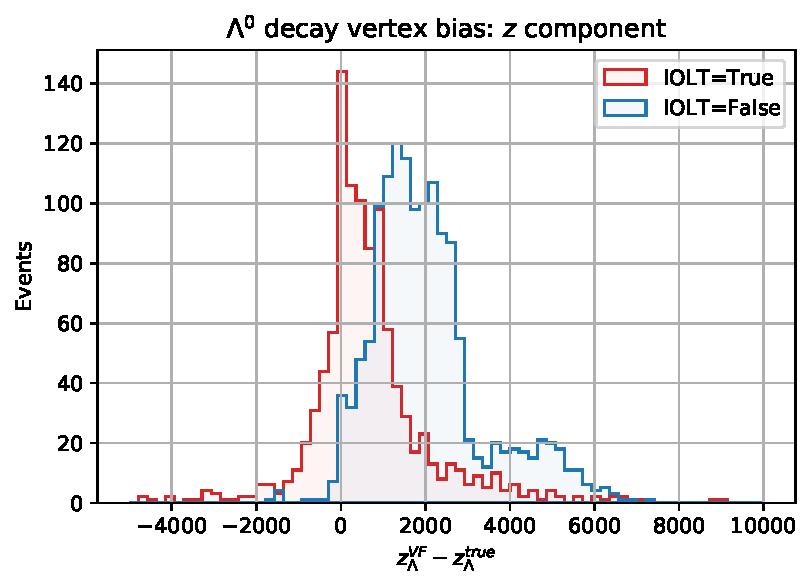
\includegraphics[width=.6\textwidth]{graphics/03-vertex_reconstruction/iolt_lambda_endvertex_z_bias.pdf}
%	\caption{A.}
%\end{figure}

As outlined in Section \ref{sec:oscillation}, vertexing failures in the $\Lambda^0 \rightarrow p\pi^-$ decay can be attributed to candidate vertices in different planes providing conflicting information.
In order to circumvent this phenomenon, my proposal for the recovery of these failed events involves performing a refit process with a slightly altered version of the standard Vertex Fitter, designed to give more importance to tracks lying on a specific plane.

The obvious choice for said plane is the $yz$ plane, since extrapolation of these tracks does not need to be concerned with magnet bending and is therefore expected to be less prone to error.
However, this would penalize events with poor $yz$ protoparticle reconstruction, for instance events with parallel or diverging tracks in said plane.
To maximize the recovery efficiency of my solution, I have elected to perform three separate refits on non-converging events, prioritizing $yz \rightarrow xz \rightarrow xy$ planes in this order.
In a worst-case scenario, this would quadruple the time complexity of the vertexing process; in practice, half of all events converge with the standard VF, and about $\approx 15\%$ more converge after the first refit attempt ($yz$ plane).
%%@todo: stima dell'aumento del tempo

Considering the $yz$ plane as an example, we can prioritize available information for tracks in this plane by artificially increasing the uncertainty $\sigma_x$ for the $x$ component of the candidate vertex position $\vec{x}$.
At each step in a VF iteration, $\vec{x}$ is updated according to \eqref{eq:VF_new_vertex_final}.
Uncertainties enter the computation through three terms:
\begin{enumerate}
	\item $C^{-1}_{k-1}$, inverse $\vec{x}$ covariance matrix computed at the previous step (or previous iteration);
	\item ${V_r}_k^{-1}$, inverse covariance matrix of reference point $\vec{r}_k$, computed at the true transport of particle $k$;
	\item $C_k$, current $\vec{x}$ covariance matrix, inverted from the matrix sum of the previous two terms as in \eqref{eq:3:VF_new_inv_covmatrix}.
\end{enumerate}
Ergo, the best approach to increase $\sigma_x$ while minimizing additional computation time is to act on the individual components of $C^{-1}_{k-1}$ and ${V_r}_k^{-1}$ just before the \eqref{eq:3:VF_new_inv_covmatrix} sum.

Assuming gaussian uncertainties, a standard three-dimensional covariance matrix will have the form
\begin{equation}
C = \begin{pmatrix}
	\sigma_x^2 & \rho_{xy} \sigma_x \sigma_y & \rho_{xz} \sigma_x \sigma_z \\
	\rho_{xy} \sigma_x \sigma_y & \sigma_y^2 & \rho_{yz} \sigma_y \sigma_z \\
	\rho_{xz} \sigma_x \sigma_z & \rho_{yz} \sigma_y \sigma_z & \sigma_z^2 \\
\end{pmatrix},
\label{eq:3:gaussian_covmatrix}
\end{equation}
where $\rho_{ij} \coloneqq \text{corr}(i,j)$. Its inverse matrix is written as
\begin{equation}
C^{-1} = \frac{1}{K} \begin{pmatrix}
%%%%%%%%%%%%%%%%%%%%%%%%%%%%%%%%%%%
\frac{1-\rho_{yz}^2}{\sigma_x^2} &&
\frac{\rho_{xz}\rho_{yz} - \rho_{xy}}{\sigma_x \sigma_y} &&
\frac{\rho_{xy}\rho_{yz} - \rho_{xz}}{\sigma_x \sigma_z} \\
%%%%%%%%%%%%%%%%%%%%%%%%%%%%%%%%%%%
\frac{\rho_{xz}\rho_{yz} - \rho_{xy}}{\sigma_x \sigma_y} &&
\frac{1-\rho_{xz}^2}{\sigma_y^2} &&
\frac{\rho_{xy}\rho_{xz} - \rho_{yz}}{\sigma_y \sigma_z} \\
%%%%%%%%%%%%%%%%%%%%%%%%%%%%%%%%%%%
\frac{\rho_{xy}\rho_{yz} - \rho_{xz}}{\sigma_x \sigma_z} &&
\frac{\rho_{xy}\rho_{xz} - \rho_{yz}}{\sigma_y \sigma_z} &&
\frac{1-\rho_{xy}^2}{\sigma_z^2}
\end{pmatrix},
\label{eq:3:inverse_gaussian_covmatrix}
\end{equation}
with
\begin{equation}
K \coloneqq \frac{\det C}{\sigma_x^2 \sigma_y^2 \sigma_z^2} = 1+2\rho_{xy} \rho_{xz} \rho_{yz} - \rho_{xy}^2 - \rho_{xz}^2 - \rho_{yz}^2.
\end{equation}
Going back to the $yz$ plane example, we increase $\sigma_x$ by introducing a multiplicative factor $s_x < 1$ for relevant covariance matrix components as follows:
\begin{equation}
\begin{aligned}
&C^{-1}_{xx} = C^{-1}_{xx} \times s_x^2, \\
&C^{-1}_{xy} = C^{-1}_{yx} = C^{-1}_{xy} \times s_x, \\
&C^{-1}_{xz} = C^{-1}_{zx} = C^{-1}_{xz} \times s_x,
\end{aligned}
\label{eq:3:sigma_x_rescaled}
\end{equation}
with other components left as is.
This process is also applied to ${V_r}_k^{-1}$ and replicated at each step of the refit algorithm, which I'll refer to as \textit{$\sigma_x$-rescaled}.
Similarly, the $\sigma_y$-rescaled and $\sigma_z$-rescaled algorithms prioritize planes $xz$ and $xy$ respectively;
their extension from \eqref{eq:3:sigma_x_rescaled} should be trivial.
For the remainder of this section, I'll also refer to their sequential application $\sigma_x \rightarrow \sigma_y \rightarrow \sigma_z$ as the \textit{$\sigma$-rescaled refit process}, unless otherwise stated.

As proof of concept, I have analyzed the performance of the $\sigma$-rescaled refit approach with $s_i=0.98, i\in\{x,y,z\}$ (corresponding to $\approx 2\%$ increase in vertex uncertainties) on a sample of [@todo:how many] MC-generated \demonstratorshort events, observing a $+25\%$ increase in reconstructed events.
As per Figure \ref{fig:lambda_lambdab_reco_efficiency}, this amounts to about a quarter of all reconstructible events.

%% @todo: rimpiazza DTF JPsi con DTF JPsiLambda
%% @todo: sostituisci con multicolumn? Median bias: zvtx, pdtf?
\begin{table}[t]
	\begin{center}
	\begin{tabular}{@{}lllll@{}}
		\toprule
		Increased $\sigma$ & Recovery eff. & $\mu_\frac{1}{2}\left[\tilde{\chi}^2_\text{vtx}\right]$ & $\mu_\frac{1}{2}\left[z_\text{vtx}^\Lambda \text{ bias}\right]$ & $\mu_\frac{1}{2}\left[p_z^\text{DTF} (p) \text{ bias}\right]$ \\
		\midrule
		None (VF)  & -- & 1.0 & 429 mm & $+1.35\%$ \\
		$\sigma_x$ & 62\% & 4.9 & 584 mm & $-0.84\%$ \\
		$\sigma_y$ & 74\% & 5.4 & 635 mm & $-0.81\%$ \\
		$\sigma_z$ & 80\% & 7.8 & 697 mm & $-1.02\%$ \\
		Sequential & 100\% & 6.5 & 646 mm & $-0.93\%$ \\
		\bottomrule
	\end{tabular}
	\end{center}
	\caption[Performance comparison of the three rescaled-$\sigma$ algorithms.]{Performance comparison of the three rescaled-$\sigma$ algorithms with $s_i=0.98$ (see text for details), contrasted with the performance of their sequential application ($\sigma_x \rightarrow \sigma_y \rightarrow \sigma_z$) and the standard Vertex Fitter algorithm. Recovery efficiency is defined as the ratio of events reconstructed by a certain flavour over the total number of events recoverable by combining the three algorithms. $\mu_\frac{1}{2}$ identifies the median value. Performances for $xyz$ algorithms are computed using all events recovered by the individual flavour, including events recovered by more than one, while values for VF are computed on standard reconstructed events.}
	\label{tab:3:xyz_VF_performances}
\end{table}

I have also run each algorithm individually after the standard VF to gauge their performance on the $n^\text{reco}_\text{tot}$ recovered events.
Results of this test are compiled in Table \ref{tab:3:xyz_VF_performances}.
When considering the \textit{recovery efficiency} of each algorithm, defined as the fraction of recovered events converging under said algorithm, i.e.
\begin{equation}
	\varepsilon^\text{reco}_i \rvert_{i\in\{x,y,z\}} = \frac{n_i^\text{reco}}{n_\text{tot}^\text{reco}},
\end{equation}
the $\sigma_z$-rescaled is the better performing one, reaching convergence in $\approx 80\%$ of recoverable events.
Despite this, all three $\sigma$-rescaled algorithms have a sizable number of <<exclusive>> events that do not reach convergence under any other variation.
Furthermore, while the $\sigma_z$-rescaled does recover more events by itself, only $\approx 5\%$ of the total recovered events are exclusive to it, meaning its overall impact on the $\sigma$-rescaled refit process is low.

The established $\sigma_x \rightarrow \sigma_y \rightarrow \sigma_z$ refit order is justified in light of performance evaluation based on the goodness of these fits.
As seen again in Table \ref{tab:3:xyz_VF_performances}, the $\sigma_x$-rescaled algorithm has comparatively lower vertex $\tilde{\chi}^2$, $z_\text{vtx}^\Lambda$ bias and proton $p_z$ bias using the DTF algorithm with \jpsi and \lz mass constraints.
Using the $\sigma_z$-rescaled algorithm as last resort means only $\approx 5\%$ of recovered events are actually affected by its poor performance.

%\begin{figure}[t]
%	\centering
%	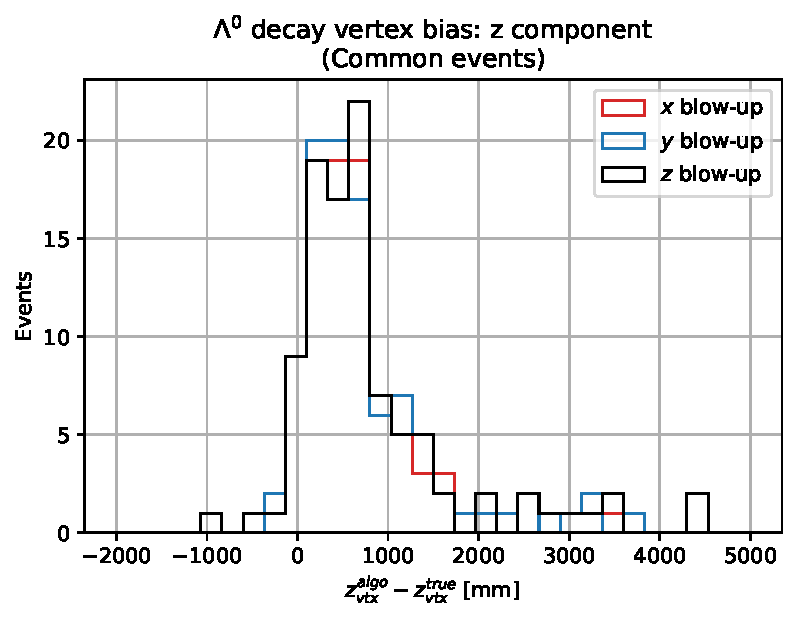
\includegraphics[width=.6\textwidth]{graphics/03-vertex_reconstruction/Lambda_endvertex_z_bias_xyz_common.pdf}
%	\caption{A.}
%	\label{fig:3:Lambda_endvertex_z_bias_xyz_common}
%\end{figure}
%
%Figure \ref{fig:3:Lambda_endvertex_z_bias_xyz_common} shows the $z_\text{vtx}^\Lambda$ bias of the individual $\sigma$-rescaled algorithms in the $\approx 36\%$ of recovered events which converge under all three variations.
%Despite the difference in performance outlined in Table \ref{tab:3:xyz_VF_performances}

\begin{figure}[t]
	\centering
	\begin{subfigure}{.45\textwidth}
		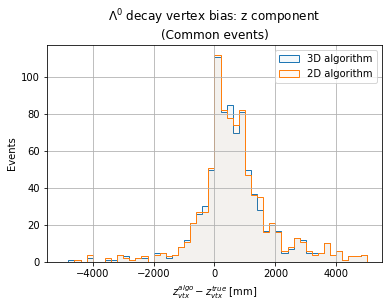
\includegraphics[width=\textwidth]{graphics/03-vertex_reconstruction/3D_vs_2D_lambda_endvertex_bias_common.png}
		\caption{}
		\label{fig:3:3D_vs_2D_lambda_endvertex_bias_common}
	\end{subfigure}
	\begin{subfigure}{.45\textwidth}
		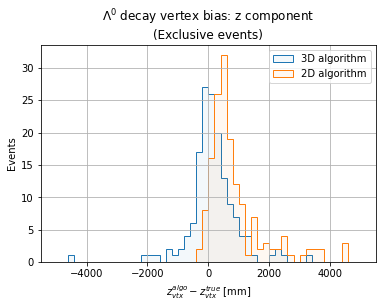
\includegraphics[width=\textwidth]{graphics/03-vertex_reconstruction/3D_vs_2D_lambda_endvertex_bias_exclusive.png}
		\caption{}
		\label{fig:3:3D_vs_2D_lambda_endvertex_bias_exclusive}
	\end{subfigure}
	\caption[A and b.]{Left right}
	\label{fig:3:3D_vs_2D_lambda_endvertex_bias_common_vs_exclusive}
\end{figure}

All $\sigma$-rescaled algorithms still appear to perform significantly worse than the standard VF on all the above fronts.
To investigate this, I have individually run the $\sigma_x$-rescaled and standard VF algorithms on all available events and compared their results.
Considering the total number of events reconstructed by combining the two, $\approx 74\%$ of them are reconstructed by both, $\approx 13\%$ are only reconstructed by the $\sigma_x$-rescaled (these are the $\sigma_x$-recovered events from Table \ref{tab:3:xyz_VF_performances}) and a roughly equal $\approx 13\%$ of them are only reconstructed by the Vertex Fitter.

What's more interesting is the performance comparison. Figure \ref{fig:3:3D_vs_2D_lambda_endvertex_bias_common} shows the $z_\text{vtx}^\Lambda$ bias on events common to VF and $\sigma_x$-rescaled.
Despite the median \SI{15}{\centi\meter} discrepancy reported in Table \ref{tab:3:xyz_VF_performances}, the two distributions are indistinguishable from the other.
The expected difference only emerges when considering events exclusive to each algorithm, as seen in Figure \ref{fig:3:3D_vs_2D_lambda_endvertex_bias_exclusive}.

The differences in $z_\text{vtx}^\Lambda$ and proton $p_z^\text{DTF}$ bias are therefore to be understood in terms of what events reach convergence with a specific algorithm, rather than as performance evaluations of the algorithm itself.
The $\sigma_x$-rescaled algorithm does not intrinsically reconstruct events with larger bias;
instead, its $yz$-centric approach allows it to recover events that throw off the standard VF, and these events tend to have a larger $z_\text{vtx}^\Lambda$ bias on their best vertex candidate.
This tendency is likely the result of the systematic T track $p_z$ underestimation analyzed in Section \ref{sec:3:kinematics_at_first_meas}.

\begin{figure}[t]
	\centering
	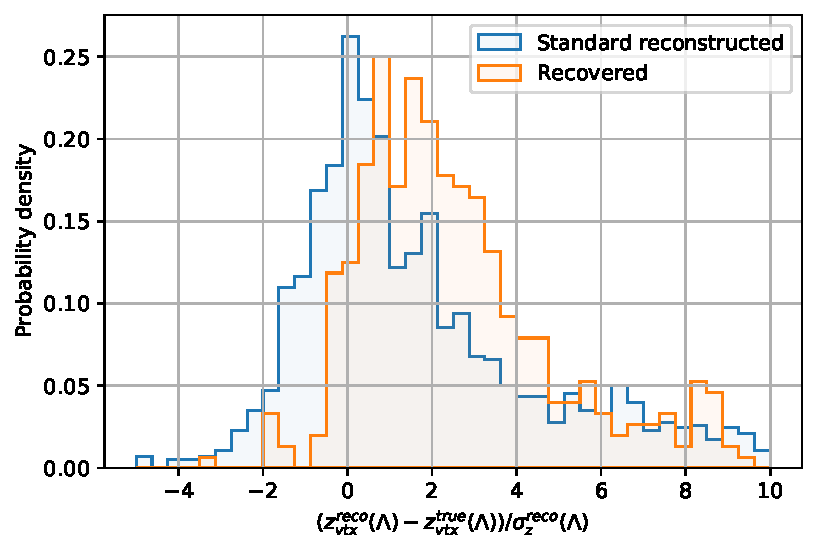
\includegraphics[width=.6\textwidth]{graphics/03-vertex_reconstruction/xyz_L_ENDVERTEX_residual_2Dv3D_z_rel.pdf}
	\caption{A.}
	\label{fig:3:xyz_L_ENDVERTEX_residual_2Dv3D_z_rel}
\end{figure}

Overall, my $\sigma$-rescaled refit process proposal allows for the recovery of an extra $+25\%$ of signal events.
While $\tilde{\chi}^2_\text{vtx}$ and bias on $z_\text{vtx}^\Lambda$ are higher compared to events reconstructed via Vertex Fitter (see Figure \ref{fig:3:xyz_L_ENDVERTEX_residual_2Dv3D_z_rel} and Table \ref{tab:3:xyz_VF_performances}), there is sufficient evidence pointing towards this being a problem intrinsic to the non-converged events themselves.
Their impact on the prospective \lz EDM/MDM measurement will have to be evaluated in dedicated sensitivity studies and possibly incorporated as a source of systematic uncertainty to be accounted for.

%%@todo: se trovi un posto adatto, menziona che xyz insieme non fungono. Non è che sia importante.
%% Problema: deve essere grassetto nella ToC e nel titolo del capitolo, ma non grassetto nell'header.
\chapter{Signal event selection}
\label{cap:event_selection}

\section{Prefiltering}
\label{sec:prefilter}
\textit{Prefilters}, also refered to as \textit{preliminary selections} or simply \textit{pre-selections}, are the foundation of the signal selection process.
The main objective of this step is to improve the signal-to-background ratio and reduce the computational workload to analyze data with cuts on kinematic variables.

\begin{table}[t]
	\begin{center}
	\begin{tabular}{@{}llll@{}}
		\toprule
		Variable & Unit & Minimum & Maximum \\
		\midrule
		$p(p)$ 						& MeV/$c$ 	& 2\,000	& 500\,000 \\
		$p_T(p)$ 					& MeV/$c$ 	& 400		& -- \\
		$p(\pi^-)$ 					& MeV/$c$ 	& 10\,000	& 500\,000 \\
		$z_\Lambda^\text{vtx}$		& mm		& 5\,500	& 8\,500 \\
		$p_T(\Lambda^0)$ 			& MeV/$c$ 	& 450		& -- \\
		$m(p\pi^-)$	(Vertex Fitter)	& MeV/$c^2$	& 600		& 1\,500 \\
		$m(p\pi^-)$	(combined)		& MeV/$c^2$	& --		& 2\,000 \\
		$m(p\pi^-)$	(measured)		& MeV/$c^2$	& --		& 1\,500 \\
		$\cos\xi_p (\Lambda^0)$		& --		& 0.9999	& -- \\
		$\Delta \chi^2_\text{PV} (\Lambda^0)$
									& -- 		& --		& 200 \\
		$\chi^2_\text{dist} (\Lambda^0)$
									& --		& --		& $2\times{10}^{7}$ \\
		$\chi^2_\text{vtx} (\Lambda^0)$
									& --		& --		& 750 \\
		$\lvert m(\mu^+ \mu^-) - m_\text{PDG} (J/\psi) \rvert$
									& MeV/$c^2$ & --		& 90 \\
		$m(J/\psi~\Lambda^0)$ (combined)
									& MeV/$c^2$	& 4\,700		& -- \\
		$m(J/\psi~\Lambda^0)$ (Vertex Fitter)
									& MeV/$c^2$	& --		& 8\,500 \\
		$\lvert \cos\xi_p (\Lambda^0_b) \rvert$
									& --		& 0.99		& -- \\
		$\Delta \chi^2_\text{PV} (\Lambda^0_b)$
									& -- 		& --		& 1\,750 \\
		$\chi^2_\text{vtx} (\Lambda^0_b)$
									& --		& --		& 150 \\
		\bottomrule
	\end{tabular}
	\end{center}
	\caption{Prefilter selection criteria applied to simulated \demonstratorshort signal and Run 2 data. The Vertex Fitter invariant mass is computed by the homonymous algorithm; the \textit{combined} invariant mass is computed from the 4-momenta of the daughter particles at the first measurement position, without track extrapolation; the \textit{measured} invariant mass is computed in the same way as the combined mass, but after extrapolation at the reconstructed decay vertex of the mother particle. Angle $\xi_p$ for a particle is computed between the line connecting its origin and decay vertices and the direction of its momentum. $\Delta \chi^2_\text{PV} (\Lambda^0)$ is the increase of the primary vertex $\chi^2$ when the particle is included in the fit. $\chi^2_\text{dist}$ is the geometrical distance between the primary vertex and the particle decay vertex in $\chi^2$ units.}
	\label{tab:4:prefilters}
\end{table}

\begin{figure}[t]
	\centering
	\begin{subfigure}{.45\textwidth}
		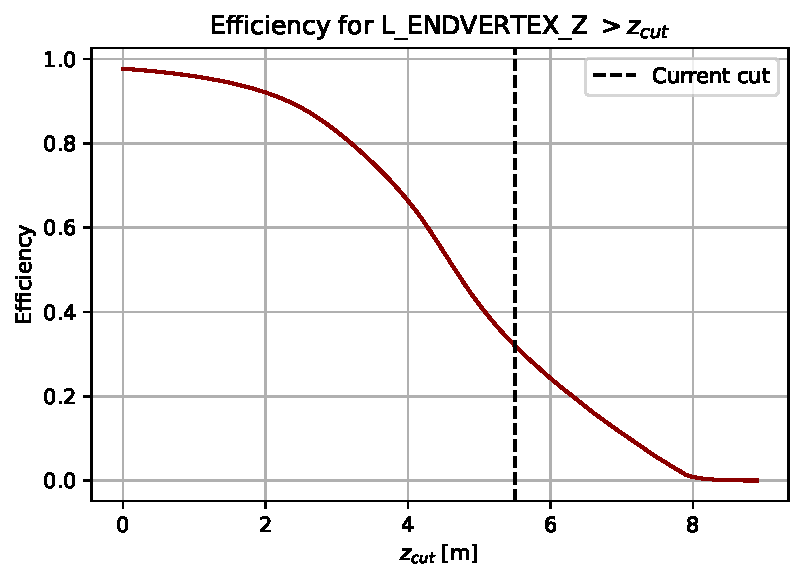
\includegraphics[width=\textwidth]{graphics/04-event_selection/LEVz_left.pdf}
		\caption{}
	\end{subfigure}
	\begin{subfigure}{.45\textwidth}
		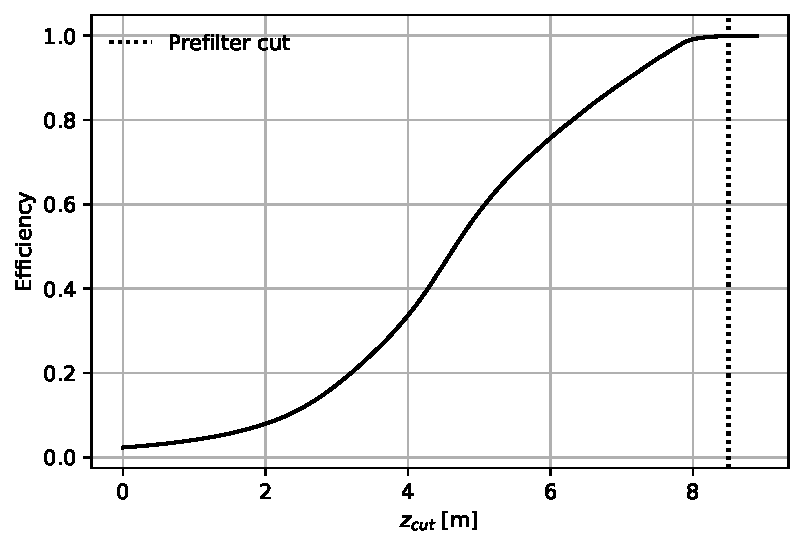
\includegraphics[width=\textwidth]{graphics/04-event_selection/LEVz_right.pdf}
		\caption{}
	\end{subfigure}
	\caption{Efficiency of the $z_\text{vtx}^\Lambda \geq z_\text{cut}^\text{left}$ \textit{(a)} and $z_\text{vtx}^\Lambda \leq z_\text{cut}^\text{right}$ \textit{(b)} prefilter selection criteria on \demonstratorshort simulated signal, as function of the respective thresholds. The \textit{dotted vertical lines} mark the chosen thresholds.}
	\label{fig:4:z_lambda_cuts}
\end{figure}

The applied prefilter criteria are listed in Table \ref{tab:4:prefilters}.
Efficiencies on signal have been estimated with studies on simulated \demonstratorshort events.
The most impactful selection is the one applied to $z_\text{vtx}^\Lambda$, the $z$ component of the \lambdadecay decay vertex;
the efficiencies for the left and right cuts as a function of the threshold are shown in Figure \ref{fig:4:z_lambda_cuts}.
Since I require $\Lambda^0$ to decay after the dipole magnet in order to observe spin precession, the [@todo] efficiency of the $z_\text{vtx}^\Lambda \geq \SI{5.5}{\meter}$ cut cannot be avoided.
Other selections have a much lower impact on signal, with efficiencies $\gtrsim 80\%$, resulting in a total prefilter efficiency of [@todo].

As detailed in Section \ref{sec:2:tracking}, a key aspect of my analysis is the employment of T tracks for the reconstruction of the \lz.
The low residual magnetic field for protons and pions produced far from the dipole magnet lowers momentum resolution for the associated tracks down to $20\% \div 30\%$.
Resolution can be improved up to $\approx 10\%$ by placing kinematic constraints on $p\pi^-$ and $\mu^+ \mu^-$ invariant masses, fixing them to the PDG values of $m(\Lambda^0)$ and $m(J/\psi)$ respectively (these will be henceforth referred to as \textit{mass constraints}).
This approach cannot be implemented in the leaf-by-leaf framework of the default Vertex Fitter algorithm for vertex reconstruction;
instead each event is refitted with the Decay Tree Fitter (DTF) algorithm in two configurations (single $J/\psi$ and double $J/\psi~\Lambda^0$ mass constraints (see also Section \ref{sec:3:dtf}).

A convergence requirement of the DTF algorithm with the $J/\psi~\Lambda^0$ mass constraints is therefore added to the prefilter selections.
The main drawback of this selection, a much steeper [@todo] efficiency on simulated signal events, is outweighed by the benefits of the improved momentum resolution in the determination of the angular distribution of \lambdadecay decay products.


\subsection{Reconstruction of \texorpdfstring{\lz}{Lambda} decay vertex in prefiltered events}
\label{sec:lambda_endvertex_bias}

The quality of the \lambdadecay vertex reconstruction affects many aspects of the $\Lambda^0$ electromagnetic dipole moments measurement:
on top of being fundamental to evaluate how much magnetic field the particle traversed (and thus the extent of spin precession), even the best momentum resolution for protons and pions is worthless if the particles are extrapolated at the wrong point of production.
Both $x_\text{vtx}^\Lambda$ and $y_\text{vtx}^\Lambda$ are fairly well reconstructed in prefiltered events, with resolution $\lesssim \SI{1}{\centi\meter}$ and no discernible bias.
This section will therefore focus on the reconstruction of $z_\text{vtx}^\Lambda$.

\begin{figure}[t]
	\centering
	\begin{subfigure}{.45\textwidth}
		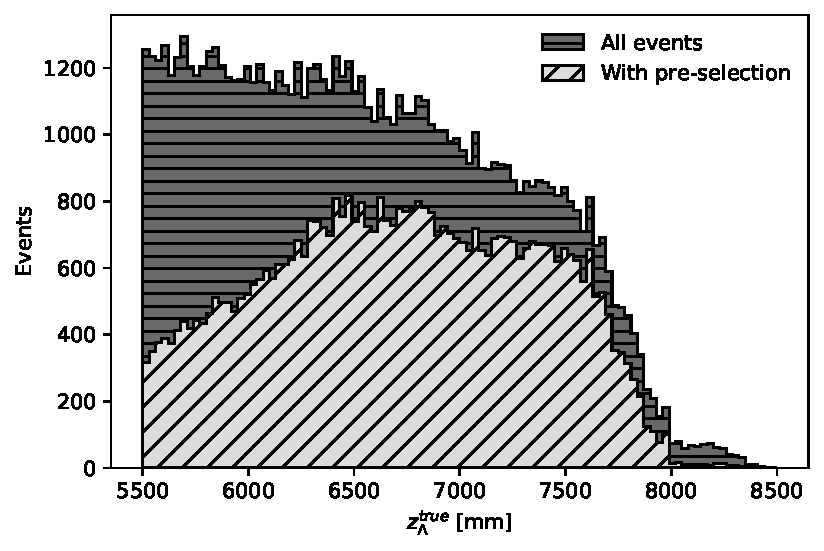
\includegraphics[width=\textwidth]{graphics/04-event_selection/Lambda_endvertex_z_true.pdf}
		\caption{}
		\label{fig:4:lz_vertex_true}
	\end{subfigure}
	\begin{subfigure}{.45\textwidth}
		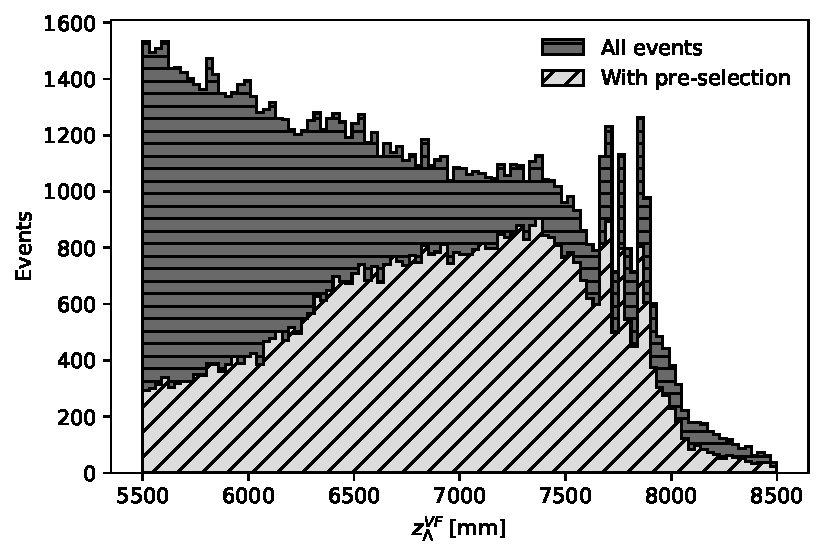
\includegraphics[width=\textwidth]{graphics/04-event_selection/Lambda_endvertex_z.pdf}
		\caption{}
		\label{fig:4:lz_vertex_reco}
	\end{subfigure}
	\caption{Distribution of true \textit{(a)} and reconstructed \textit{(b)} $z_\text{vtx}^\Lambda$ in simulated \demonstratorshort signal events, without (\textit{dark grey}) and with (\textit{light grey}) prefiltering.}
	\label{fig:4:lz_vertex_distributions}
\end{figure}

\begin{figure}[t]
	\centering
	\begin{subfigure}{.45\textwidth}
		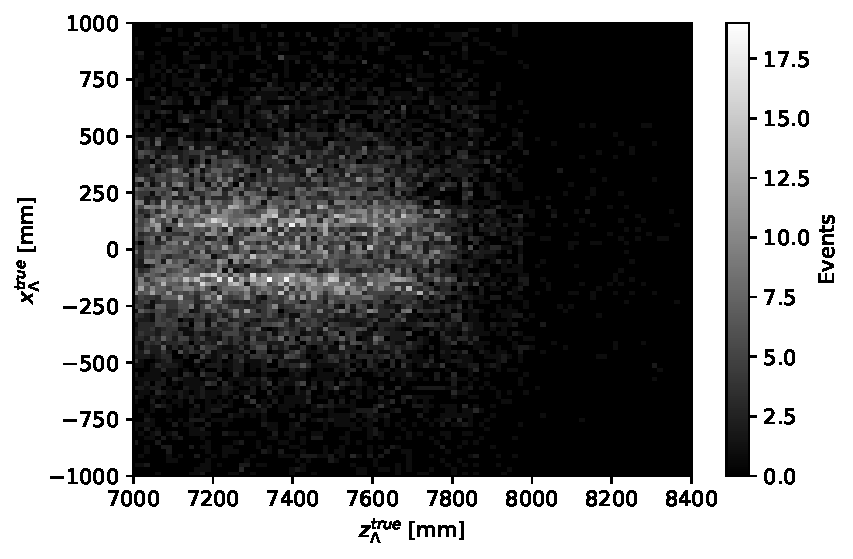
\includegraphics[height=.2\textheight]{graphics/04-event_selection/Lambda_endvertex_z_vs_x_true.pdf}
		\caption{}
		\label{fig:4:lz_vertex_peaks_true}
	\end{subfigure}
	\begin{subfigure}{.45\textwidth}
		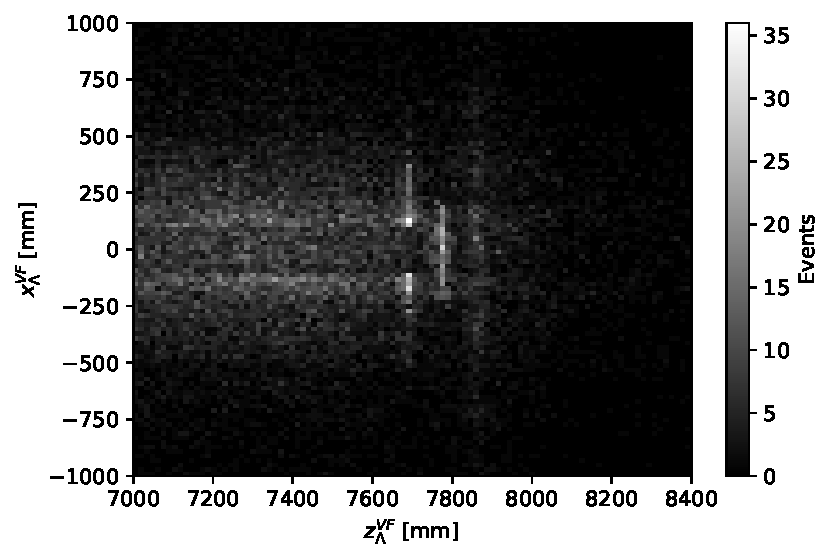
\includegraphics[height=.2\textheight]{graphics/04-event_selection/Lambda_endvertex_z_vs_x.pdf}
		\caption{}
		\label{fig:4:lz_vertex_peaks_reco}
	\end{subfigure}
	\caption{Distribution of simulated \demonstratorshort signal events (prefilters applied) with $z_\Lambda^\text{VF} \geq \SI{7.0}{\meter}$, as function of true (\textit{left}) and reconstructed (\textit{right}) $x_\Lambda^\text{vtx}$ and $z_\text{vtx}^\Lambda$. This corresponds to a top view of true and reconstructed \lz decay vertices.}
	\label{fig:4:lz_vertex_peaks}
\end{figure}

Figures \ref{fig:4:lz_vertex_true} and \ref{fig:4:lz_vertex_reco} show the distributions of true and reconstructed $z_\text{vtx}^\Lambda$ respectively for simulated signal events.
The most prominent difference between the two is the presence of three peaks in the $[\SI{7.5}{\meter},\SI{8.0}{\meter}]$ region of the reconstructed distribution, being found both with and without prefilter selections. 
The significance of these structures can be inferred by plotting the events as function of  $z_\text{vtx}^\Lambda$ and $x_\text{vtx}^\Lambda$, corresponding to a bending plane perspective of the detector.
This is shown in Figure \ref{fig:4:lz_vertex_peaks_reco}, highlighting the fact that the peaks in $\Lambda^0$ decay vertices have a very precise geometrical location, absent when comparing the true $z_\text{vtx}^\Lambda$ and $x_\text{vtx}^\Lambda$ values for the same events (Figure \ref{fig:4:lz_vertex_peaks_true}).
The spatial distribution of the vertices bears a striking resemblance to the layout of a T tracking station (see Figure \ref{fig:2:t_station_top}) and $z$ coordinates are consistent with the nominal placement of IT and first OT plane of the T1 station \cite{Barbosa-Marinho:582793}.
While dedicated studies are required to gain more insight into the source of these structures, they are assumed to be of minor impact for the purposes of this thesis.

\begin{figure}[t]
	\centering
	\begin{subfigure}{.45\textwidth}
		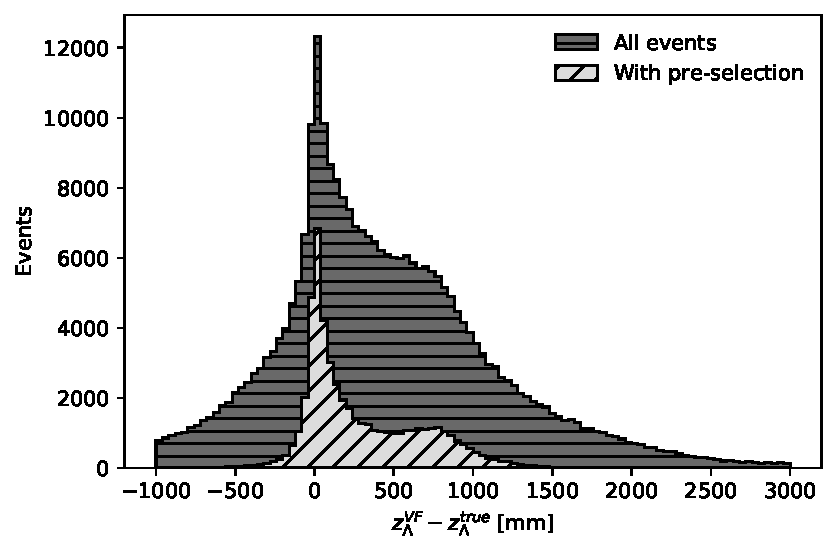
\includegraphics[width=\textwidth]{graphics/04-event_selection/Lambda_endvertex_bias_z.pdf}
		\caption{}
		\label{fig:4:lz_endvertex_bias_linear}
	\end{subfigure}
	\begin{subfigure}{.45\textwidth}
		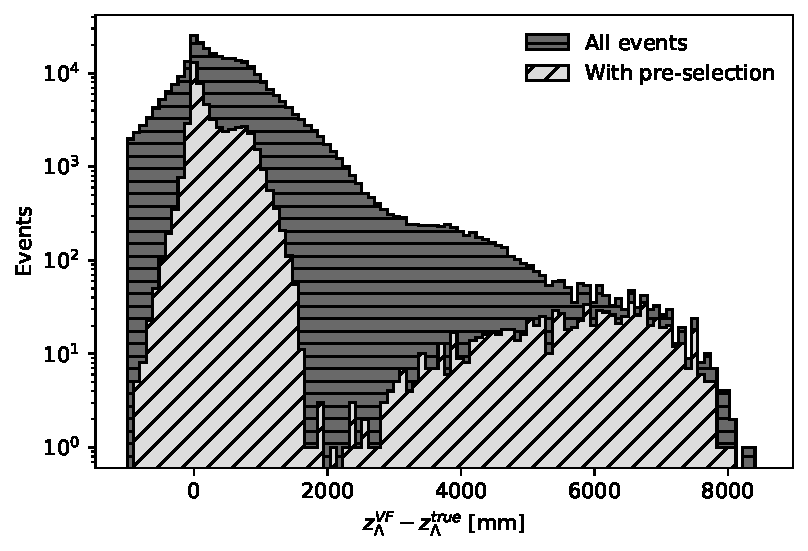
\includegraphics[width=\textwidth]{graphics/04-event_selection/Lambda_endvertex_bias_z_log.pdf}
		\caption{}
		\label{fig:4:lz_endvertex_bias_log}
	\end{subfigure}
	\caption{Distribution of $z_\text{vtx}^\Lambda$ bias for simulated \demonstratorshort events in linear \textit{(a)} and logarithmic \textit{(b)} scales, without (\textit{dark grey}) and with (\textit{light grey}) prefiltering.}
	\label{fig:4:lz_endvertex_bias}
\end{figure}

The differing shapes of true and reconstructed $z_\text{vtx}^\Lambda$ distributions from Figure \ref{fig:4:lz_vertex_distributions} are also evidence of bias effects in the \lambdadecay vertex reconstruction.
This is confirmed in Figure \ref{fig:4:lz_endvertex_bias_linear}, showing the distribution of $z_\text{vtx}^\Lambda$ bias for simulated signal events:
the shape is distinctly non-gaussian, with a long tail towards the positive end of the axis counterbalancing the expected $\approx 0$ peak.
The resulting median bias is $\approx \SI{44}{\centi\meter}$.

\begin{figure}[t]
	\centering
	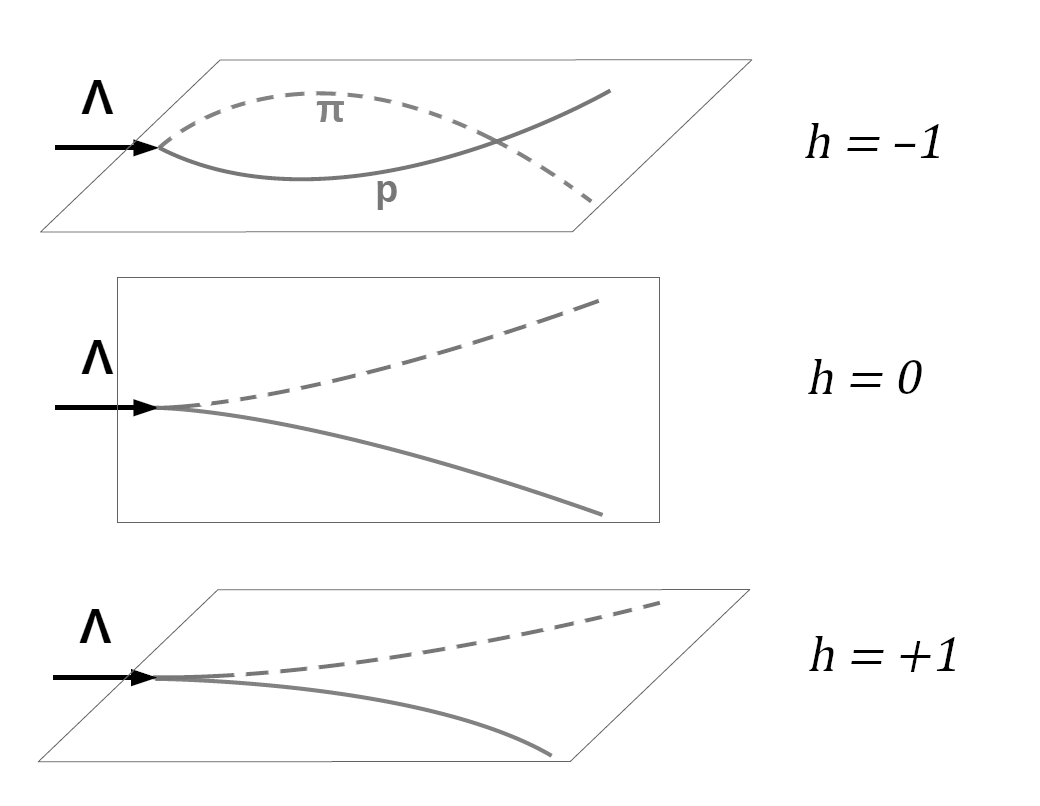
\includegraphics[width=.7\textwidth]{graphics/04-event_selection/horizontality_illustration_bw.png}
	\caption{Deptiction of three \lambdadecay configurations and the associated horizontality values. The horizontal planes in the top and bottom diagrams are aligned to the LHCb $xz$ plane, the vertical plane in the middle diagram to the $yz$ plane.}
	\label{fig:4:horizontality_explanation}
\end{figure}

The positive bias tail can be interpreted as a mistake the vertexing algorithm commits when confronted with a specific decay geometry.
When the \lambdadecay decay plane closely aligns with the $xz$ bending plane, the bending induced by the magnet can produce either \textit{opening} or \textit{closing} tracks (depicted in top and bottom diagrams respectively in Figure \ref{fig:4:horizontality_explanation}.
In the latter case the tracks will cross again at $z>z_\text{vtx}^\Lambda$;
if $y$ displacement is sufficiently small, the algorithms converges on this <<ghost>> vertex instead of the real one.

\begin{figure}[t]
	\centering
	\begin{subfigure}{.45\textwidth}
		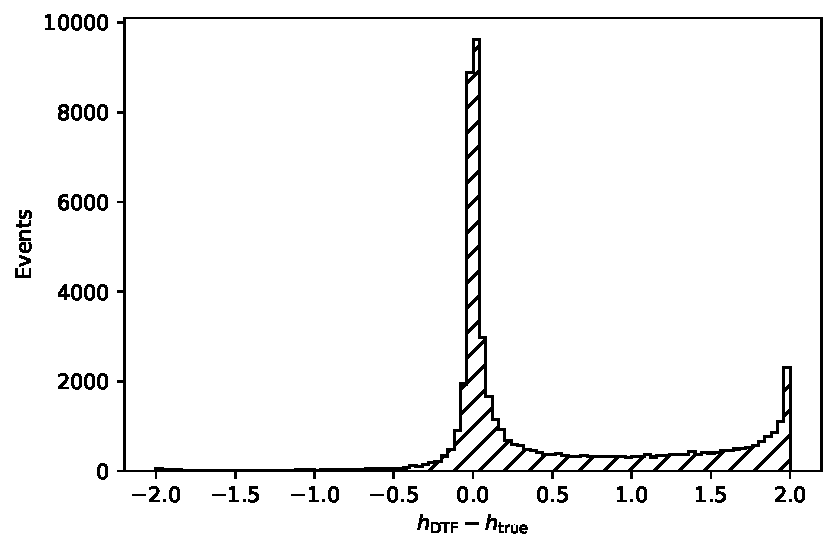
\includegraphics[width=\textwidth]{graphics/04-event_selection/Lambda_horizontality_bias.pdf}
		\caption{}
		\label{fig:4:horizontality_bias}
	\end{subfigure}
	\begin{subfigure}{.45\textwidth}
		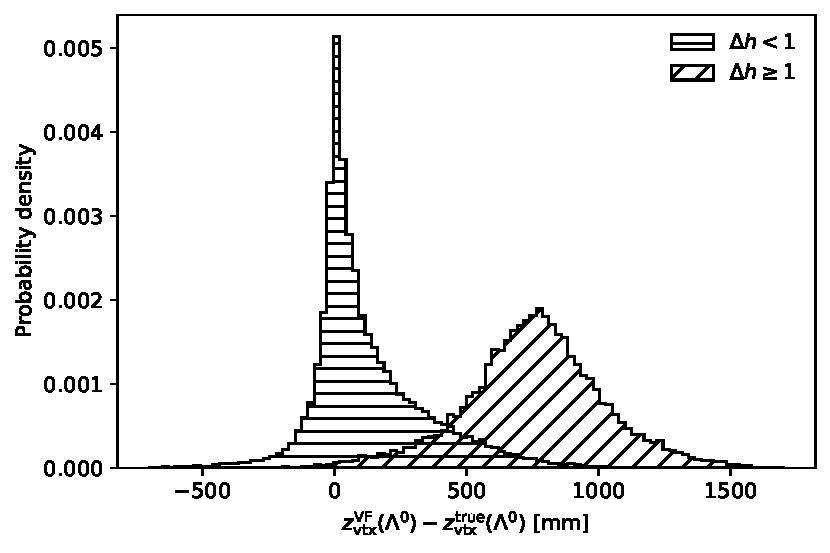
\includegraphics[width=\textwidth]{graphics/04-event_selection/lambda_endvertex_z_bias_vs_horizontality_bias.pdf}
		\caption{}
		\label{fig:4:lz_endvertex_bias_vs_horizontality_bias}
	\end{subfigure}
	\caption{\textit{(a)} Horizontality bias distribution for simulated \demonstratorshort events (prefilters applied), comparing results from Decay Tree Fitter algorithm with \jpsi and \lz mass constraints with true values. \textit{(b)} Distribution of $z_\text{vtx}^\Lambda$ bias for events with horizontality bias $<1$ (\textit{horizontal hatching}) and $\geq 1$ (\textit{diagonal hatching}).}
\end{figure}

To test out this hypothesis we define the \textit{horizontality} of a \lambdadecay event as follows:
\begin{equation}
h = \sign{\left(\Lambda^0_\text{PID}\right)} \sign{\left(B_y\right)}~\frac{a_y}{\lvert \vec{a} \rvert},
\label{eq:4:horizontality}
\end{equation}
where
\begin{equation}
\vec{a} \coloneqq \vec{p}_p \times \vec{p}_\pi 
\end{equation}
is the cross product of proton and pion momenta at production vertex, $\sign{\left(B_y\right)}$ is the dipole magnet polarity\footnote{The LHCb dipole magnet polarity is reversed roughly twice per month to allow for studies on decay asymmetries \cite{Vesterinen:1642153}. The $B_y > 0$ configuration is conventionally known as \textit{magnet up} polarity, $B_y < 0$ as \textit{magnet down}.}
and $\sign{\left(\Lambda^0_\text{PID}\right)}$ is the sign of the PDG Monte Carlo particle numbering scheme of the mother particle ($+1$ for $\Lambda^0$, $-1$ for $\bar{\Lambda}^0$) \cite{PDG}.

Decays with $h=\pm1$ lie exactly on the $xz$ bending plane, $h=-1$ events having closing $p\pi^-$/$\bar{p}\pi^+$ tracks and $h=+1$ events having opening tracks, while $h=0$ events lie on the $yz$ plane (see Figure \ref{fig:4:horizontality_explanation}).
A horizontality bias $\Delta h \coloneqq h_\text{reco} - h_\text{true} > 1$ thus becomes the signature of a <<ghost>> vertex \lambdadecay event.
As per Figure \ref{fig:4:horizontality_bias}, this issue affects $\approx 25\%$ of reconstructed \demonstratorshort events, most of those being $\Delta h \approx 2$ events (from $h=-1$ to $h=+1$), with almost no event with $\Delta h < -1$.

Isolating $\Delta h \geq 1$ events and studying their $z_\text{vtx}^\Lambda$ bias distributions (Figure \ref{fig:4:lz_endvertex_bias_vs_horizontality_bias}), it becomes clear that they are largely responsible for the high bias observed in Figure \ref{fig:4:lz_endvertex_bias_linear}.
Significant asymmetry effects are still visible in the $\Delta h < 1$ distribution, which is still skewed towards positive bias.
While not ideal, this is somewhat expected given that the Vertex Fitter algorithm scans for candidate vertices starting from the first measurement position (i.e. the T1--T3 stations) and moving upstream.

\begin{figure}[t]
	\centering
	\begin{subfigure}{.45\textwidth}
		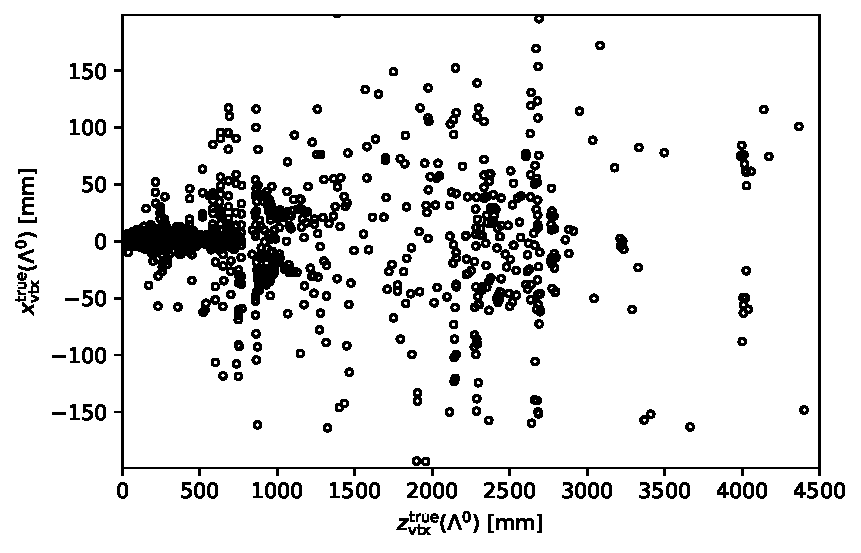
\includegraphics[width=\textwidth]{graphics/04-event_selection/bump_Lambda_true_endvertex_z_vs_x.pdf}
		\caption{}
		\label{fig:4:bump_true}
	\end{subfigure}
	\begin{subfigure}{.45\textwidth}
		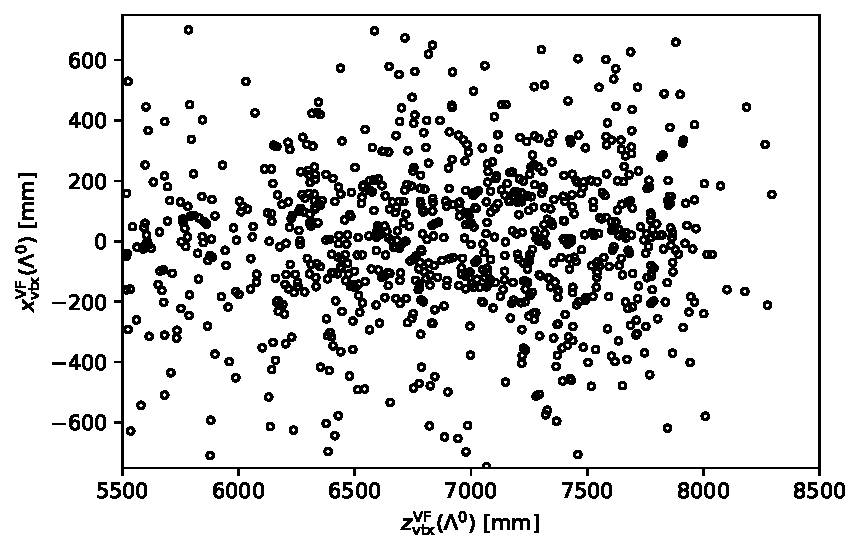
\includegraphics[width=\textwidth]{graphics/04-event_selection/bump_scatter_Lambda_endvertex_z_vs_x.pdf}
		\caption{}
		\label{fig:4:bump_reco}
	\end{subfigure}
	\caption{Distribution of simulated \demonstratorshort events (prefilters applied) with $z_\Lambda^\text{VF} - z_\Lambda^\text{true} \geq \SI{2.0}{\meter}$ as function of true \textit{(a)} and reconstructed \textit{(b)} $x_\Lambda^\text{vtx}$ and $z_\text{vtx}^\Lambda$. This corresponds to a top view of true and reconstructed \lz decay vertices.}
	\label{fig:4:bump}
\end{figure}

Most \demonstratorshort events, even those with ghost vertex reconstruction, still maintain a limited $\lesssim \SI{1.0}{\meter}$ bias on $z_\text{vtx}^\Lambda$.
A smaller substructure with $\geq \SI{2.0}{\meter}$ bias emerges when plotting the distribution in logarithmic scale, as in Figure \ref{fig:4:lz_endvertex_bias_log}.
Figure \ref{fig:4:bump_true} provides a top view of the $\Lambda^0$ decay vertices of these evemts, showing the distribution of true $z_\text{vtx}^\Lambda$ and $x_\text{vtx}^\Lambda$.
Most $\Lambda^0$ in high bias events decay in the earlier sections of the detector ($z<\SI{3.0}{\meter}$);
the high spatial concentration in specific regions of the $xz$ plane, such as the <<wings>> around $z\approx \SI{1.0}{\meter}$, as well as the consistency between the placement of these structures and the location of the different LHCb subdetectors (cf. Figure \ref{fig:2:lhcb_diagram}), suggest that they may be the result of interaction with the material.

No selection on reconstructed variables is possible to filter this class of events:
Figure \ref{fig:4:bump_reco} shows that the $\Lambda^0$ vertices are reconstructed in seemingly arbitrary positions.
Their impact on the overall performance on signal is nevertheless neglectable, since this events amount to roughly [@todo] of the total simulated sample.

\section{Physical background veto}
\label{sec:4:phys_bkg}
%Most physics analyses conducted with hadron colliders are up against two different sources of background with the same (or similar) final state as the searched signal:
%\begin{enumerate}
%	\item \textit{combinatorial} background denotes events where the particles are produced 
%	\item \textit{physical} background denotes events where 
%\end{enumerate}

The main source of physical background for the \demonstratorfull decay is the similar
\begin{equation}
	B^0 \rightarrow J/\psi~(\rightarrow \mu^+ \mu^-)~K_S^0~(\rightarrow \pi^+ \pi^-).
\end{equation}
The final states of the two decays only differ for a $p \leftrightarrow \pi^+$ change.
The $K_S^0$ meson also has a similar mean lifetime to the $\Lambda^0$, thus we expect a sizeable number of $K_S^0$ decaying after the dipole magnet.
To top it off, the masses of $K_S^0$ ([@todo]) and $B^0$ ([@todo]) are very close to those of $\Lambda^0$ ([@todo]) and $\Lambda_b^0$ ([@todo]) \cite{PDG}, muddying the waters in invariant mass fits.

As discussed in Section \ref{sec:2:pid}, the LHCb detector employs the two RICH systems to identify and distinguish between protons, pions and kaons;
in the case of $\Lambda^0$ decaying after the dipole magnet RICH1 contributions is impossible, but information from RICH2 would still be available for the vast majority of the decays at hand.
However, this is where the experimental nature of physics analyses with T tracks becomes relevant once again:
due to technical issues in the implementation, RICH2 information for particle identification is unavailable for T tracks recorded during LHC Runs 1 and 2\footnote{A large effort by the Milan and Valencia LHCb research groups is underway at the time of writing to implement RICH2 information in T track trigger lines for Run 3.}, making \physbkgshort discrimination much more difficult.

\label{sec:B0_veto}
\begin{figure}[t]
	\centering
	\begin{subfigure}{.45\textwidth}
		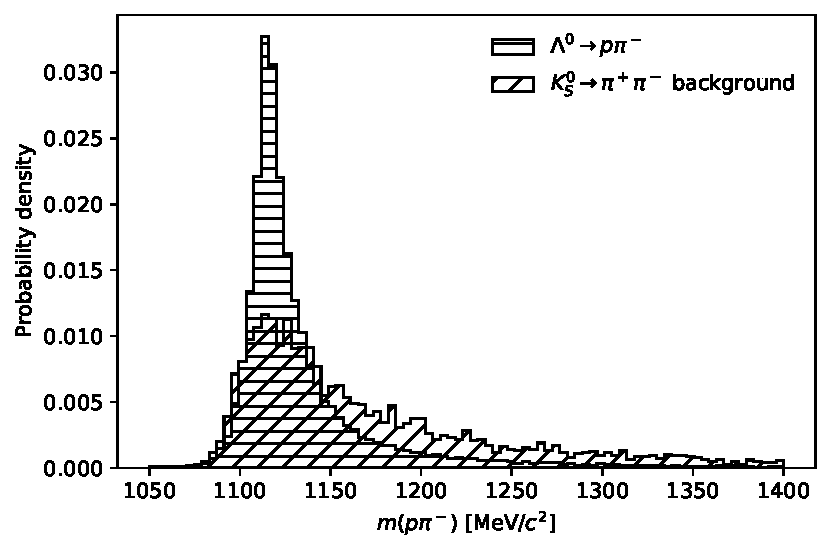
\includegraphics[width=\textwidth]{graphics/04-event_selection/phys_bkg_lambda_comparison.pdf}
		\caption{}
	\end{subfigure}
	\begin{subfigure}{.45\textwidth}
		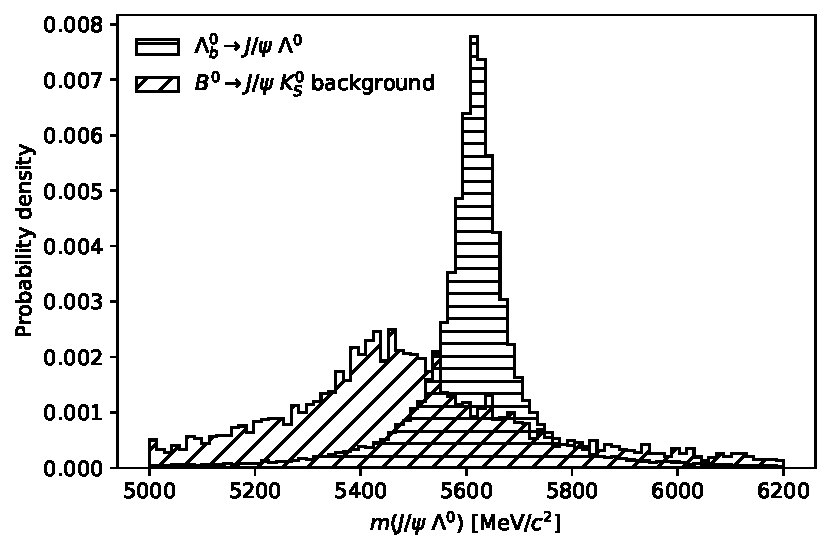
\includegraphics[width=\textwidth]{graphics/04-event_selection/phys_bkg_lambdab_comparison.pdf}
		\caption{}
	\end{subfigure}
	\caption{Comparison of simulated $m(p\pi^-)$ \textit{(a)} and $m(J/\psi~\Lambda^0)$ \textit{(b)} distributions: \demonstratorshort signal is labeled by \textit{horizontal hatching}, \physbkgshort physical background with $\pi^+ \rightarrow p$ mass hypothesis by \textit{diagonal hatching}.}
\end{figure}

\begin{figure}[t]
	\centering
	\begin{subfigure}{.45\textwidth}
		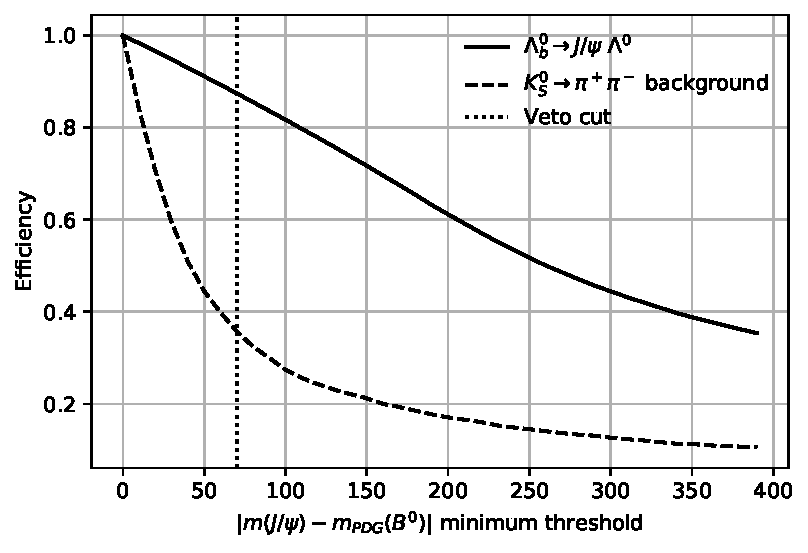
\includegraphics[height=.2\textheight]{graphics/04-event_selection/phys_veto_efficiencies.pdf}
		\caption{}
	\end{subfigure}
	\begin{subfigure}{.45\textwidth}
		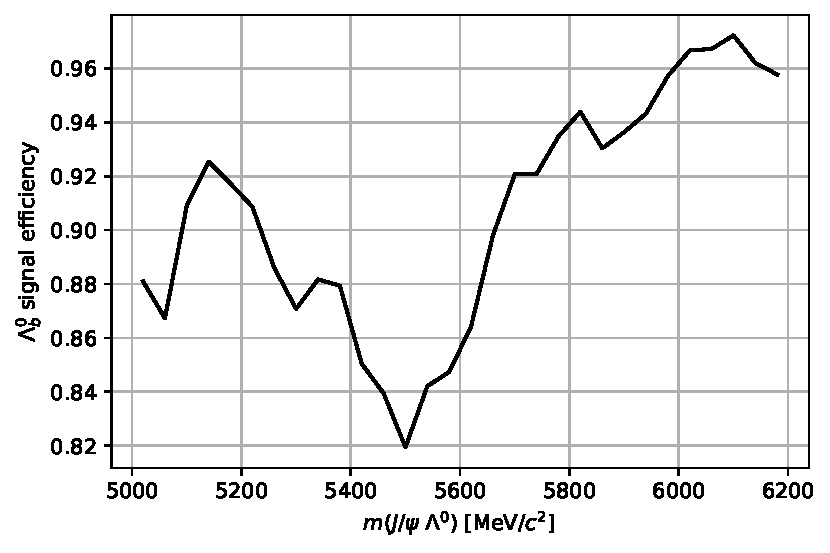
\includegraphics[height=.2\textheight]{graphics/04-event_selection/phys_veto_sig_efficiencies_per_bin.pdf}
		\caption{}
	\end{subfigure}
	\caption[Efficiency of the physical background veto as a function of the invariant mass discrepancy threshold and of $J/\psi~\Lambda^0$ invariant mass bins.]{\textit{(a)} Efficiency of physical background veto as a function of the invariant mass discrepancy threshold on simulated signal (\demonstratorshort, solid) and background (\physbkgshort with proton mass hypothesis, dashed) events. Chosen threshold marked by dotted line. \textit{(b)} Efficiency of the veto on different $m(J/\psi~\Lambda^0)$ bins for \demonstratorshort signal events).}
\end{figure}

\section{HBDT classifier}
\label{sec:HBDT}

\subsection{Training data}

\begin{figure}[t]
	\centering
	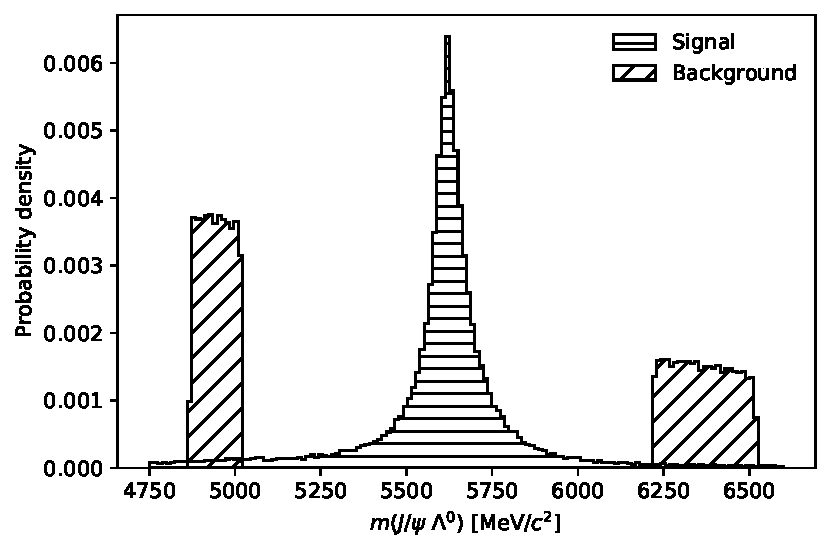
\includegraphics[width=.6\textwidth]{graphics/04-event_selection/sig_bkg_distribution_balance.pdf}
	\caption{Signal (\textit{horizontal hatching}) and background (\textit{diagonal hatching}) data samples used for training the HBDT classifier. Test samples are taken from the same pool in 1:9 ratio.}
	\label{fig:4:HBDT_training_data}
\end{figure}

\subsection{Hyperparameter optimization and performance test}
\begin{figure}[t]
	\centering
	\begin{subfigure}{.45\textwidth}
		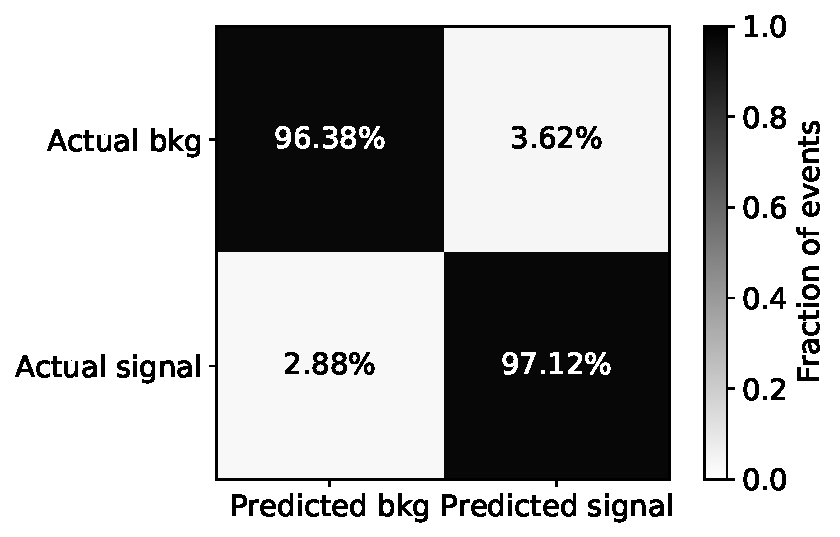
\includegraphics[width=\textwidth]{graphics/04-event_selection/confmatrix_train.pdf}
		\caption{}
	\end{subfigure}
	\begin{subfigure}{.45\textwidth}
		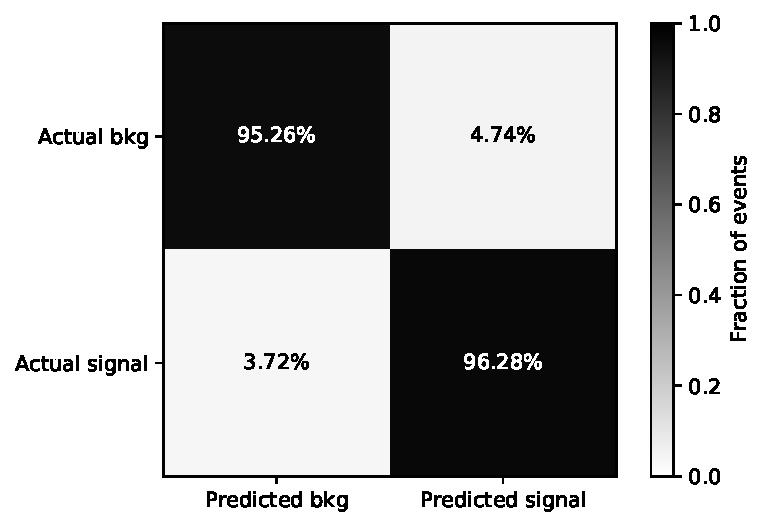
\includegraphics[width=\textwidth]{graphics/04-event_selection/confmatrix_test.pdf}
		\caption{}
	\end{subfigure}
	\caption{Confusion matrices visualizing the performance of the HBDT classifier on training \textit{(a)} and testing \textit{(b)} data samples. Percentages and chromatic scale are normalized to the true event classification: for instance, the top left and top right quadrants of a matrix represent the fraction of true background events reconstructed as background or signal, respectively. Binary classification uses an illustrative response threshold $s_\text{thres} = 0.5$.}
\end{figure}

\begin{figure}[t]
	\centering
	\begin{subfigure}{.45\textwidth}
		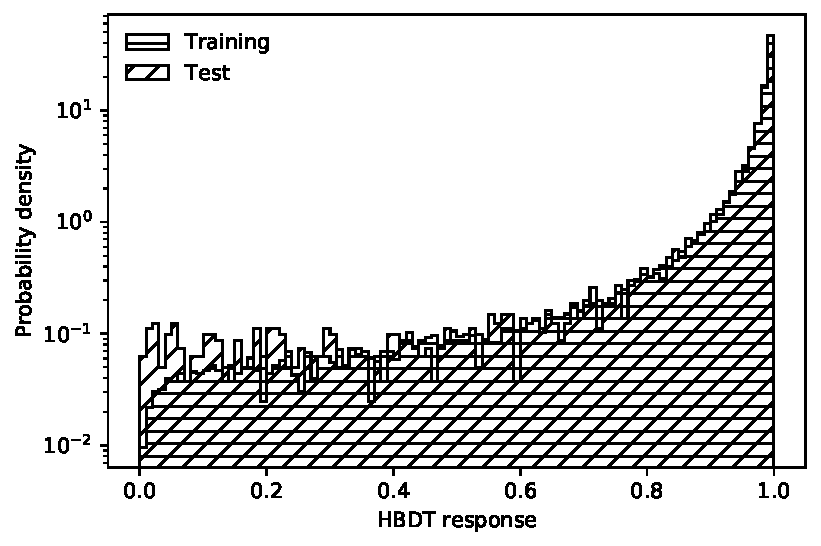
\includegraphics[width=\textwidth]{graphics/04-event_selection/sig_train_vs_test.pdf}
		\caption{}
	\end{subfigure}
	\begin{subfigure}{.45\textwidth}
		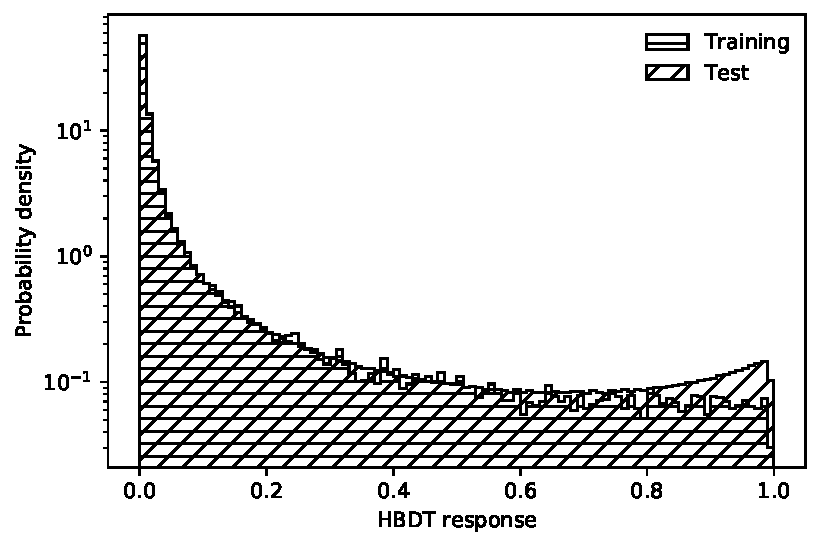
\includegraphics[width=\textwidth]{graphics/04-event_selection/bkg_train_vs_test.pdf}
		\caption{}
	\end{subfigure}
	\caption{Response distribution of the HBDT classifier on signal \textit{(a)} and background \textit{(b)} events. The training sample is represented by horizontal hatching, the test sample by diagonal hatching.}
\end{figure}

\begin{figure}
	\centering
	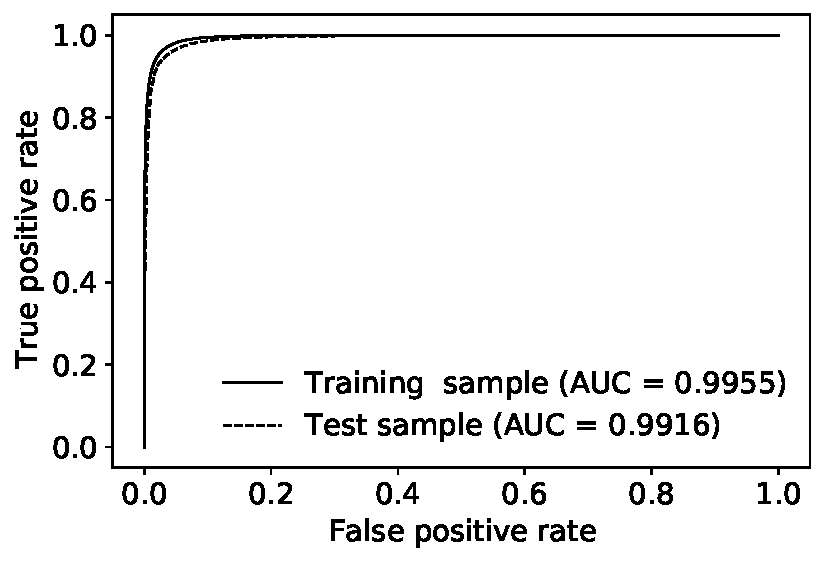
\includegraphics[width=.6\textwidth]{graphics/04-event_selection/roc.pdf}
	\caption{Receiving operating characteristic (ROC) curve for the HBDT classifier on training (\textit{solid}) and test (\textit{dashed}) samples. The legend includes the area-under-curve (AUC) score.}
\end{figure}

\subsection{Threshold optimization}

\begin{figure}
	\centering
	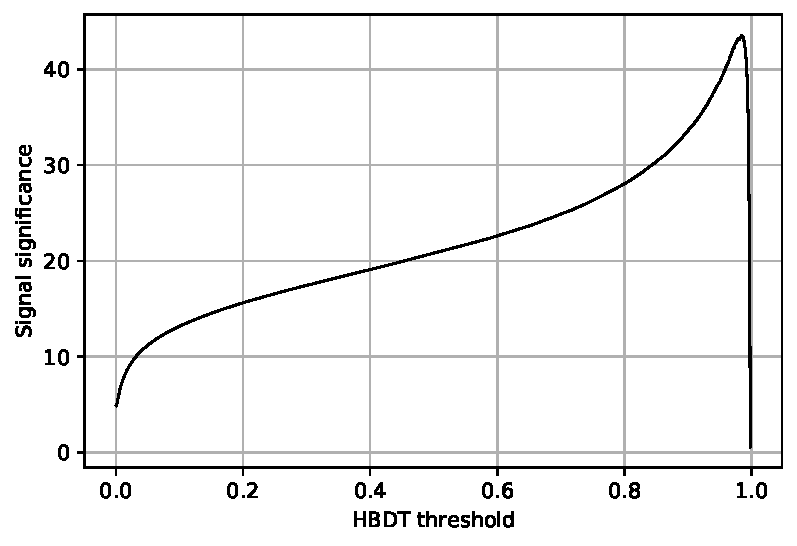
\includegraphics[width=.6\textwidth]{graphics/04-event_selection/HBDT_signal_significance.pdf}
	\caption{Projected \demonstratorshort signal significance over background as a function of the HBDT response threshold used for selection.}
\end{figure}

\section{Performance on data}
Gli invariant mass fits, essenzialmente.

\begin{figure}[t]
	\centering
	\begin{subfigure}{.45\textwidth}
		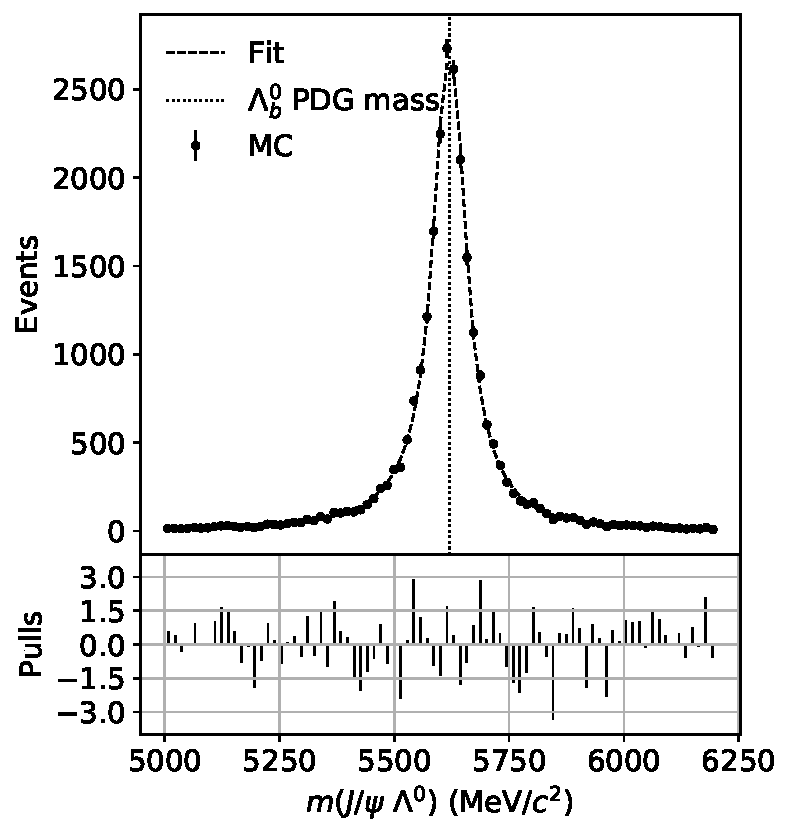
\includegraphics[width=\textwidth]{graphics/04-event_selection/MC_lambdab_hard_fit.pdf}
		\caption{}
	\end{subfigure}
	\begin{subfigure}{.45\textwidth}
		\includegraphics[width=\textwidth]{graphics/04-event_selection/data_lambdab_hard_fit.pdf}
		\caption{}
	\end{subfigure}
	\caption{Fitted $m(J/\psi~\Lambda^0)$ invariant mass distributions for simulated \demonstratorshort events \textit{(a)} and Run 2 data \textit{(b)} after all selection steps. Signal fit function is \textit{dashed}, background fit function in \textit{(b)} is \textit{dash-dotted}. The current best measurement for $\Lambda_b^0$ mass is marked by the \textit{dotted vertical line}. Fit pulls (data-fit discrepancy divided by uncertainty) are shown below the main plots.}
\end{figure}


%%%%%%%%%%%%%%%%%%%%%%%%%%%%%%%%

\appendix
%\chapter{Angular distribution of \texorpdfstring{$\Lambda \rightarrow p\pi^-$}{Lambda to proton-pion} decay products} \label{chap:angular-distribution}

\section{Helicity formalism}
[Il Richman.]

\section{Computation of the angular distribution}

%%%%%%%%%%%%%%%%%%%%%%%%%%%%%%%%

\backmatter

\bibliography{tex_files/0c-bibliography}

\end{document}
